\chapter{Design}

\section{Overall System Design}

\subsection{Short description of the main parts of the system}

\begin{flushleft}
\textbf{Main Parts of the System}
 \\ \par These are the main parts of the proposed system.
	\begin{itemize}
			\item Proposed System User Interface
			\item Adding a New Job
			\item Adding a New Client
			\item Adding a New Material
			\item Sorting and Searching Clients
			\item Removing Clients or Jobs
			\item Calculating Costs For Each Job
			\item Generating Reports
			\item Invoice Output for Client
			\item Appointment Output for Client
	\end{itemize}

\end{flushleft}


\textbf{Proposed System User Interface}
	\begin{itemize}
		\item Once onto the proposed system, the plasterer will be able to see various buttons in the action bar at the top of the program; these include Add
Jobs, Clients, Materials.
		\item Pressing the Jobs Button will then take them to a different user interface which will then display a series of other options that are applicable under the Jobs section. These include Add Job, Delete Job, Search Jobs, Edit Job. 

	\end{itemize}
\textbf{Adding a New Job}
	\begin{itemize}
		\item The plasterer will click on a + new job button on the main window and will then be shown a different layout allowing the plasterer to add the details of a new job to the database.
		\item Whilst entering the job details various validation techniques will be implemented on the data entered into the fields. For example, there will be a post code regular expression validation to make sure that the post code entered is one of a correct and valid format.
		\item Once the form has been validated and submitted the plasterer will be show a success (or failure) message to let them know that it was added ok (or not).
	\end{itemize}

\textbf{Adding a New Client}

	\begin{itemize}
		\item The user will be able to click on a + new client button that will be situated on the main window and once clicked on, the user will be shown a new layout allowing the user to enter a new client and add all of their details to the application database.
		\item Whilst entering the new client info the data that is entered will be validated and the line edit will change colour depending on whether that data entered is valid or not. For the client details there will also be a regular expression validator attached to various fields including the client phone number, client email and client post code.
		\item Once the form data has been validated and is ok the data will be committed to the database and the user will be shown a message telling them whether it added the new client to the database successfully or not. They will then be returned to the main layout.
	\end{itemize}

\textbf{Adding a New Material}

	\begin{itemize}
		\item The user will be able to add multiple materials to the database to use when calculating the cost of a job.
		\item The user will be able to click a + new material button on the main window and then will be shown a new layout allowing them to enter the details and cost etc of the new material. The data entered will also be validated.
		\item Once the new material is added a success or failure message will be displayed to the user and then they will be returned to the main layout.
	\end{itemize}

\textbf{Sorting and Searching Clients}

	\begin{itemize}
		\item The user will be able to press a "Search Clients" button on the main window and then they will be taken to a new layout showing them a table with a list of the clients and their details. 
		\item Below the table widget their  will be a search field that allows the user to search for specific clients quickly and efficiently.
		\item The results will be updated on the text Changed event.
		\item The user will be able to sort the clients not only by search but other attributes such as town/city. When the user clicks the sort by town/city push button the results will update and be sorted by town.
	\end{itemize}

\textbf{Removing Clients and Jobs}

	\begin{itemize}
		\item Removing Clients will be a feature available in the clients section of the application. The user will be able to manage the clients in a "Manage Clients" area of the application.
		\item Their will be a table widget showing a list of all the clients and when a client record is clicked various options will become available to the user such as delete or edit. 
	\end{itemize}

\textbf{Calculating Costs for each Job}

	\begin{itemize}
		\item The calculation of the job will occur once the user clicks generate invoice for a specific job.
		\item This "Generate Invoice" button will be situated within the jobs section of the application (which will be available by clicking the "Jobs" button in the main layout).
		\item By clicking "Generate Invoice" the algoritm will collaborate all the available information regarding that specific job. See the algorithm section for more detail on this algorithm.
		\item In addition to this the user (plasterer) will be able to override the resulting calculations if need be before the final details are sent to the client.
	\end{itemize}

\textbf{Generate Reports}

	\begin{itemize}
		\item The reports section will be available by clicking a "Generate Report" button that will in the Jobs section of the application. 
		\item When the generate report button has been clicked a new layout will be displayed showing a table detailing the amount of money earned in a user specified period.
		\item The time period to generate a report for will be able to be edited through a form below the report table. The form will ask where/when/who to generate a report for.
		\item Reports will be able to be generated for different plasterers and different clients; or all clients and all plasterers etc.
	\end{itemize}

\textbf{Invoice Output for Client}

	\begin{itemize}
		\item An invoice for a job will be able to be generated by clicking a "Generate Invoice" button on the specific job. 
		\item Once clicked, the invoice will be displayed on screen in a preview box and then when the user is happy with it they can click "Print Invoice" to print the invoice or "Email Invoice" to email the invoice to the client through the email stored for the client within the database.
	\end{itemize}


\textbf{Appointment Output for Client}

	\begin{itemize}
		\item The appointments will be made by clicking the "Setup Appointment" button on the specific job an appointment is needed for.
		\item When clicked, a new layout will display allowing the user to select an appointment date and time for the client.
		\item Once validated and inserted into the database, the client will be emailed a copy of the appointment details.
	\end{itemize}


\pagebreak
\subsection{System flowcharts showing an overview of the complete system}
\textbf{Flow Chart Key}
\begin{flushleft}
This is the key for the following flow charts.
\end{flushleft}
\begin{figure}[H]
    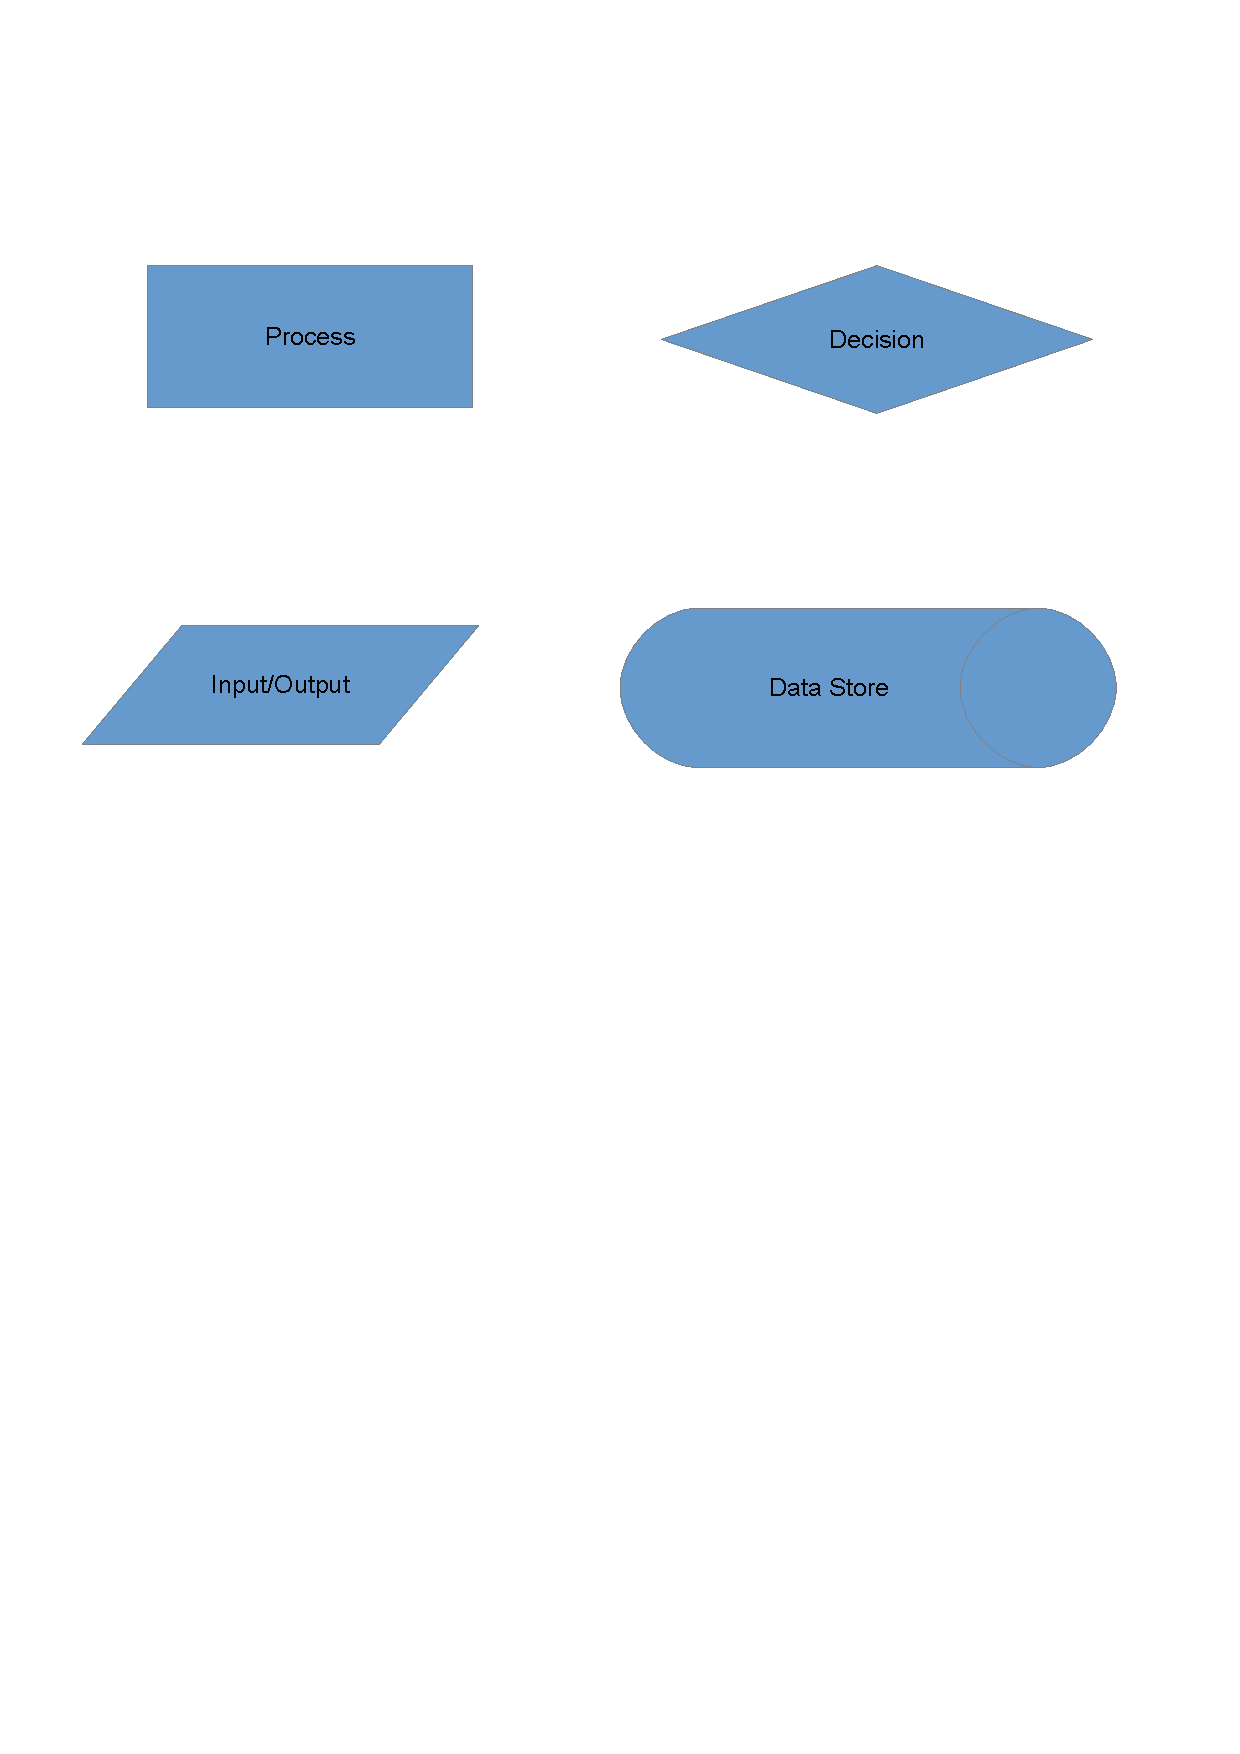
\includegraphics[scale=0.4]{./Design/images/key.pdf}
    \caption{This is the flow chart key.} \label{fig:FlowChartKey}
\end{figure}


\pagebreak
\textbf{Main Menu Flow Chart}
\begin{flushleft}
This flow chart shows the options at the main menu in the application.
\end{flushleft}
\begin{figure}[H]
    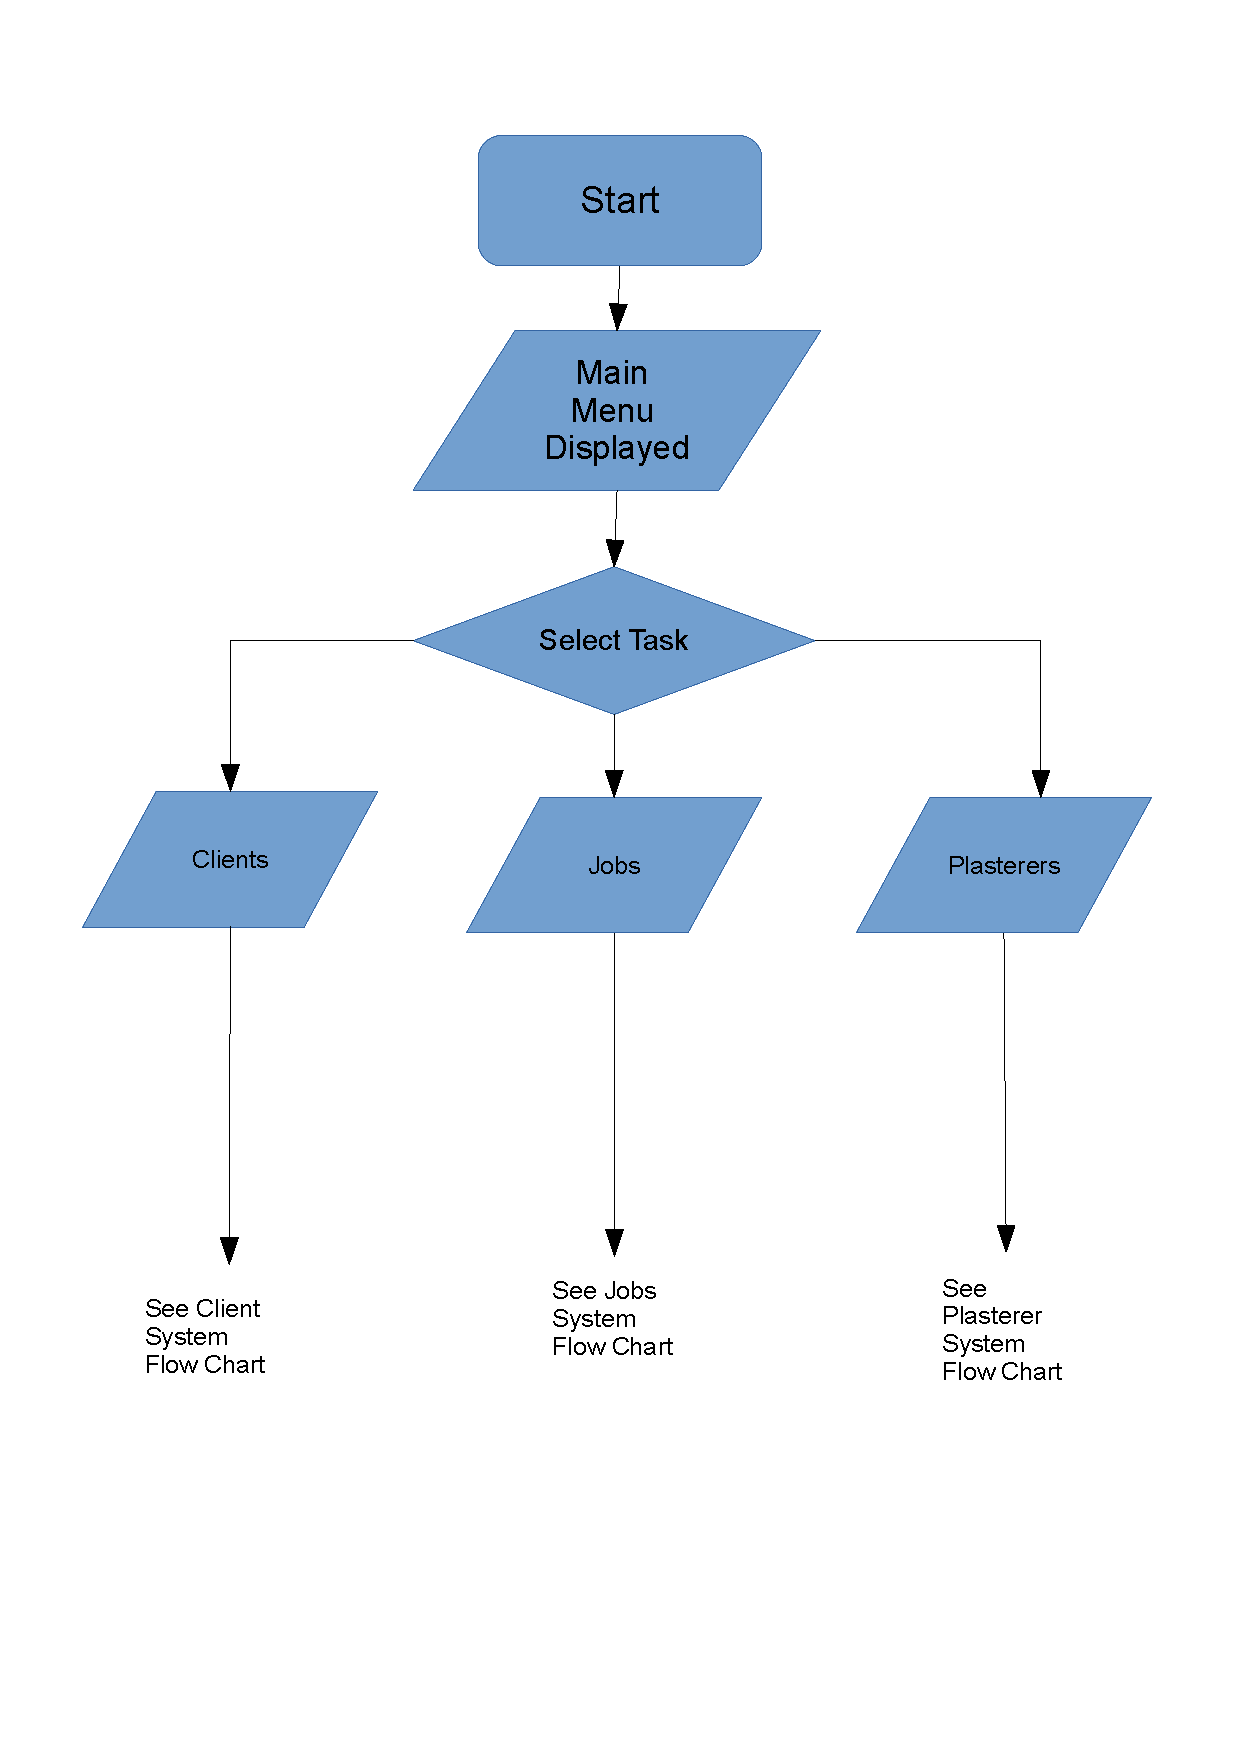
\includegraphics[scale=0.4]{./Design/images/FlowChartMainMenu.pdf}
    \caption{This is the flow chart showing the Main Menu Selection.} \label{fig:FlowChartMainMenu}
\end{figure}


\pagebreak
\underline{\textbf{Client Flow Charts}}
\begin{flushleft}
The flow charts below show the options which can be selected for clients in the application; this includes adding a new client, searching clients and editing clients.
\end{flushleft}
\textbf{Client Menu Flow Chart}
\begin{flushleft}
This is the Client Menu flow chart which shows the options to select in the application regarding clients; this includes adding a new client, searching clients and editing clients.
\end{flushleft}
\begin{figure}[H]
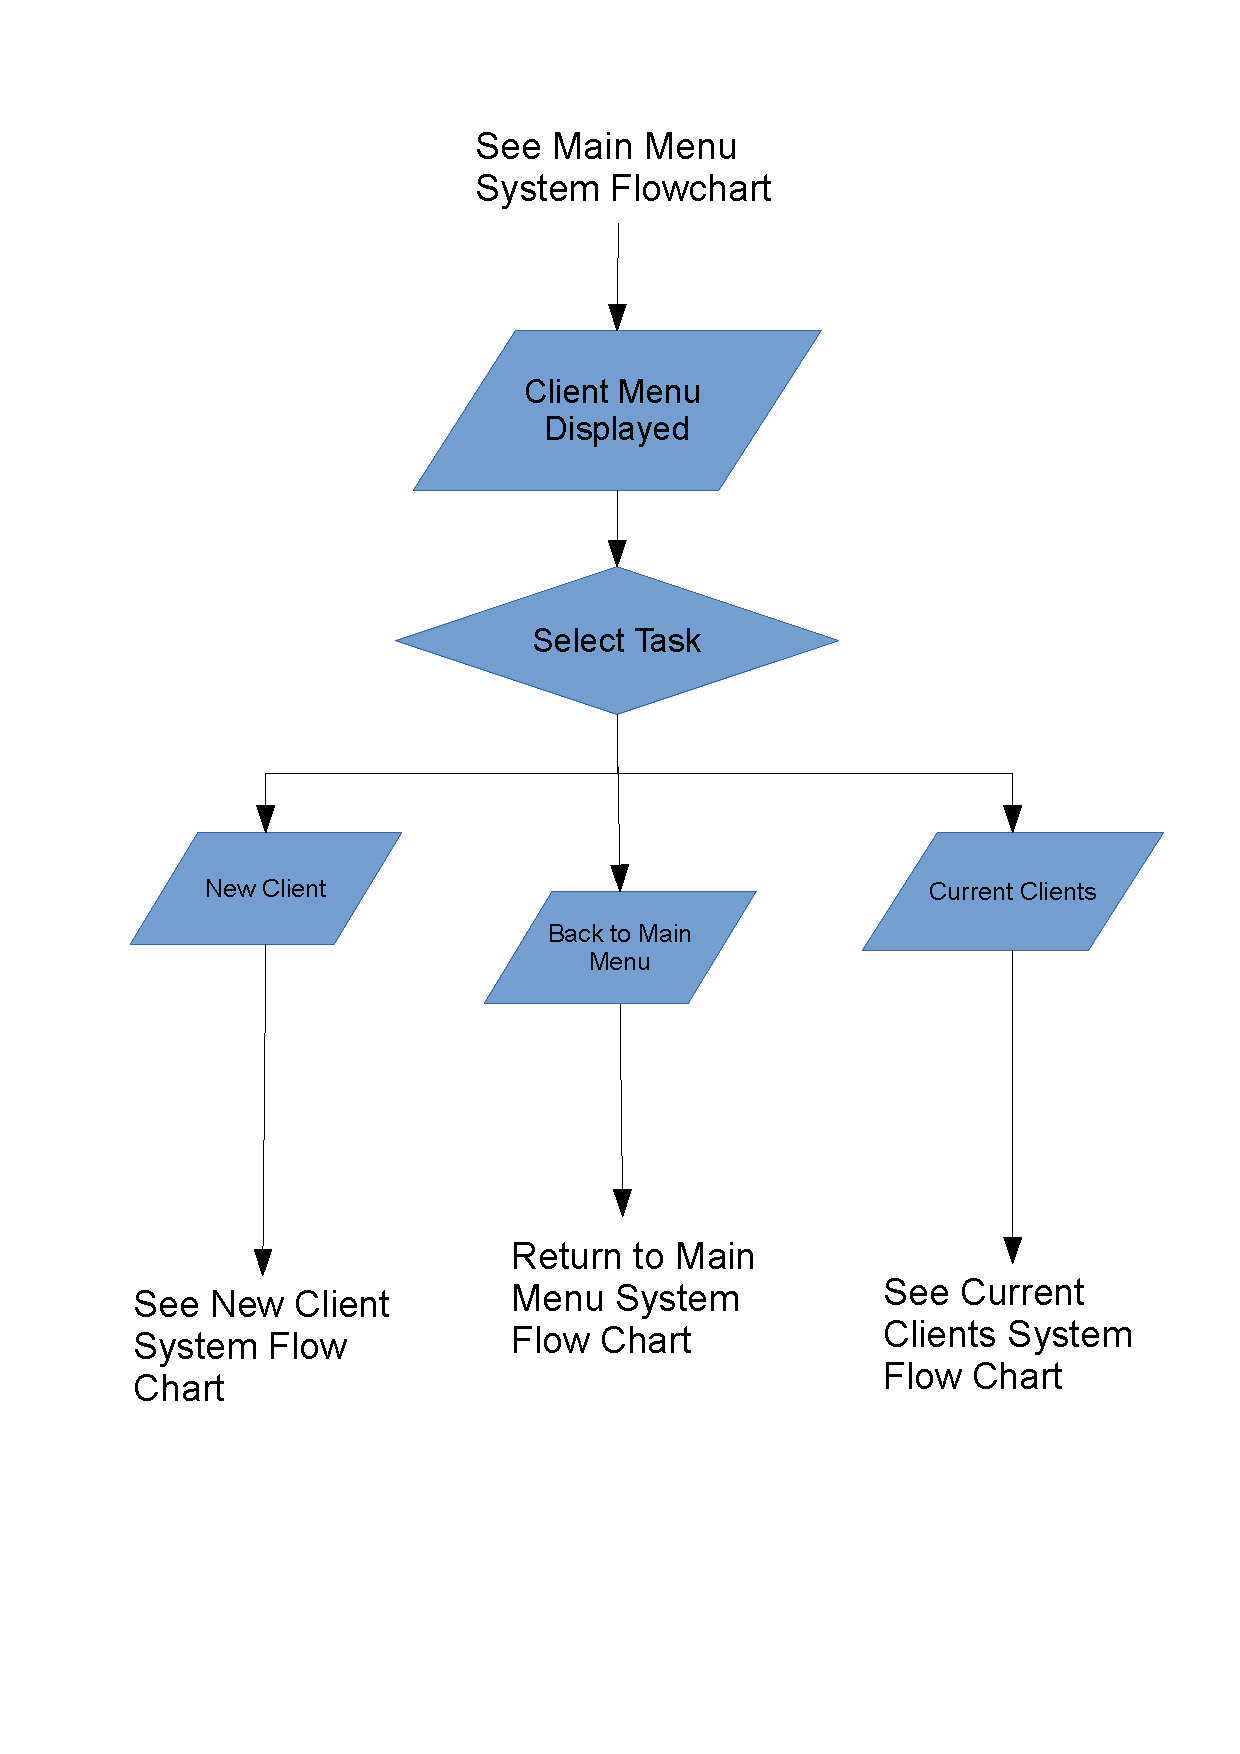
\includegraphics[scale=0.3]{./Design/images/FlowChartClientMenu.pdf}
    \caption{This is the flow chart showing the Client Menu Selection.} \label{fig:FlowChartClientMenu}
\end{figure}

\pagebreak
\textbf{New Client Flow Chart}
\begin{flushleft}
Below is a flow chart to show what happens when you add a new client in the proposed system.
\end{flushleft}
\begin{figure}[H]
    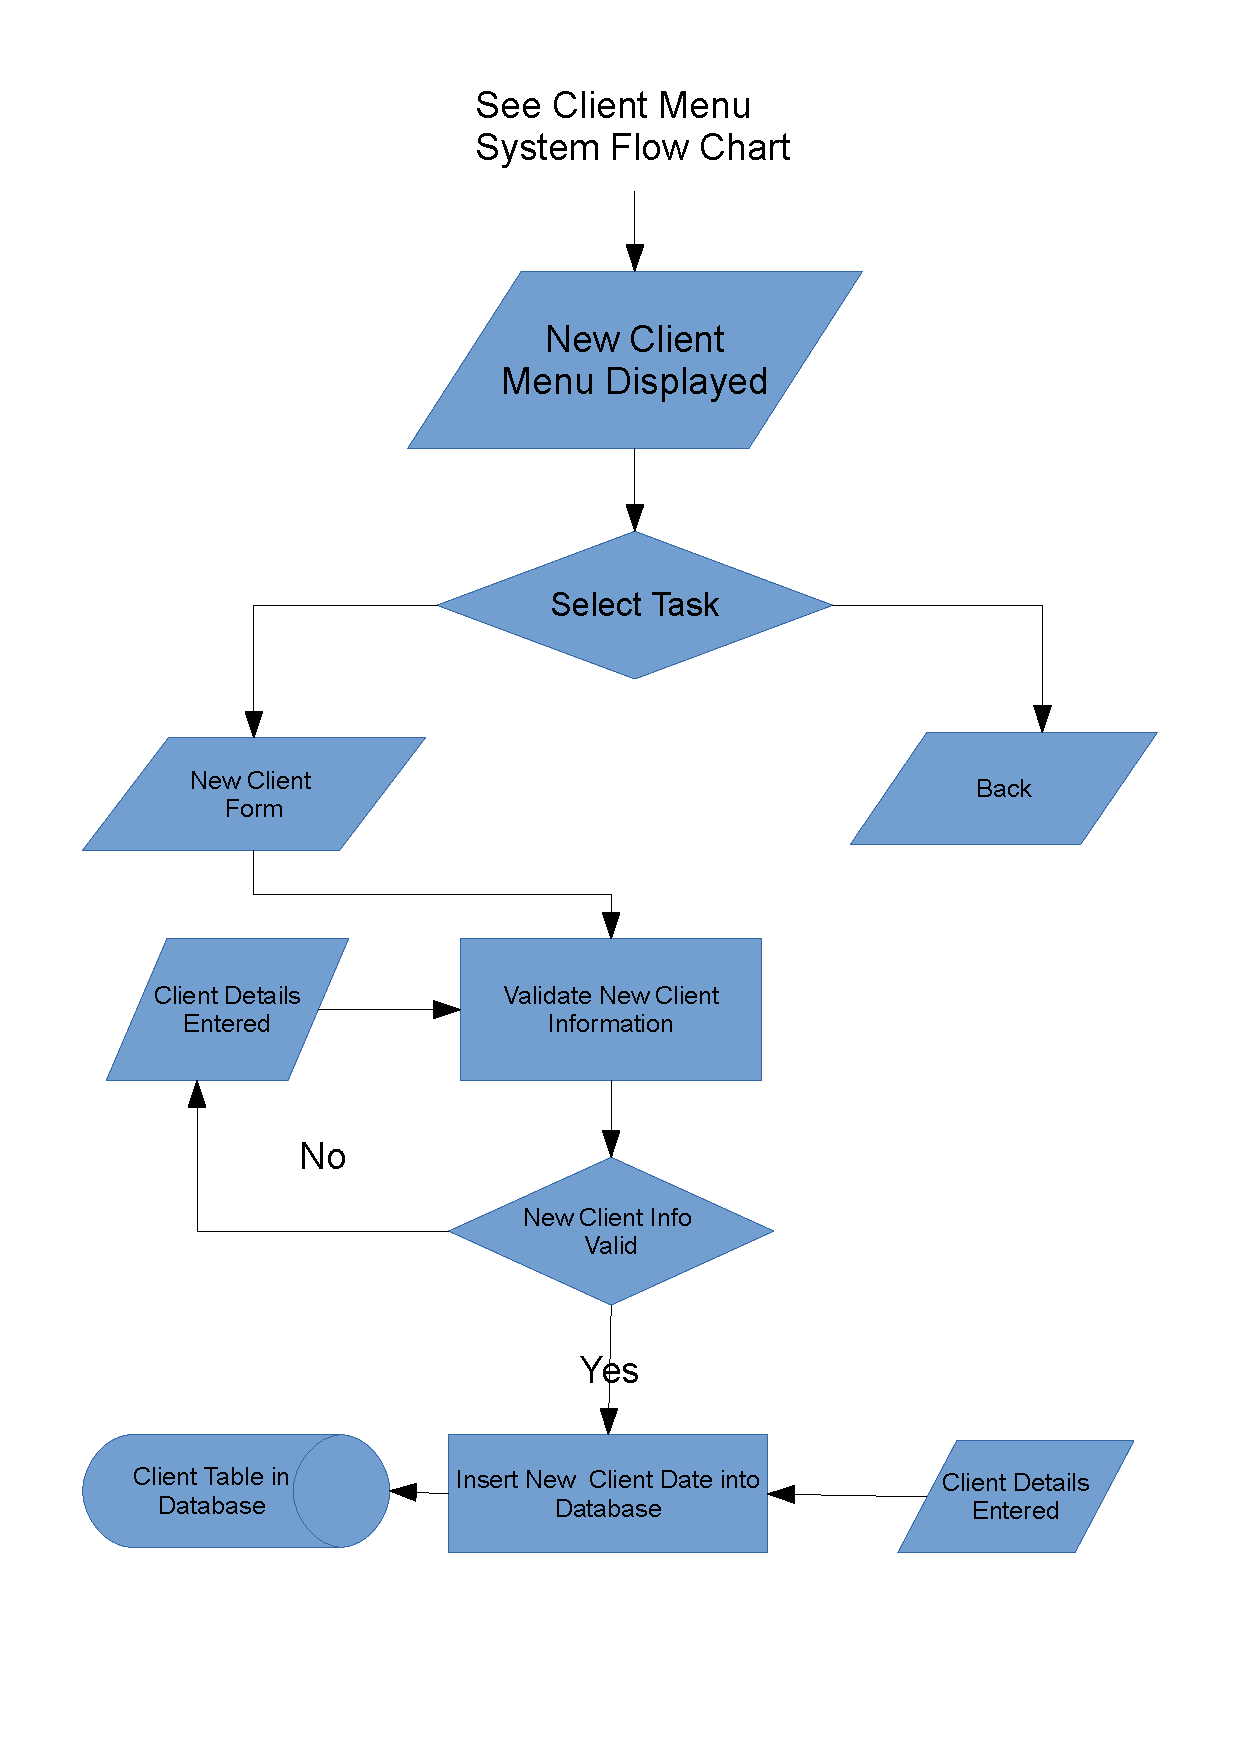
\includegraphics[scale=0.5]{./Design/images/FlowChartNewClient.pdf}
    \caption{This is the flow chart showing the addition of a new client to the proposed system.} 
\label{fig:FlowChartNewClient}
\end{figure}

\pagebreak
\textbf{Current Clients Flow Chart}
\begin{flushleft}
Below is the current clients flow chart which shows the flow of control in the proposed system for this section.
\end{flushleft}
\begin{figure}[H]
    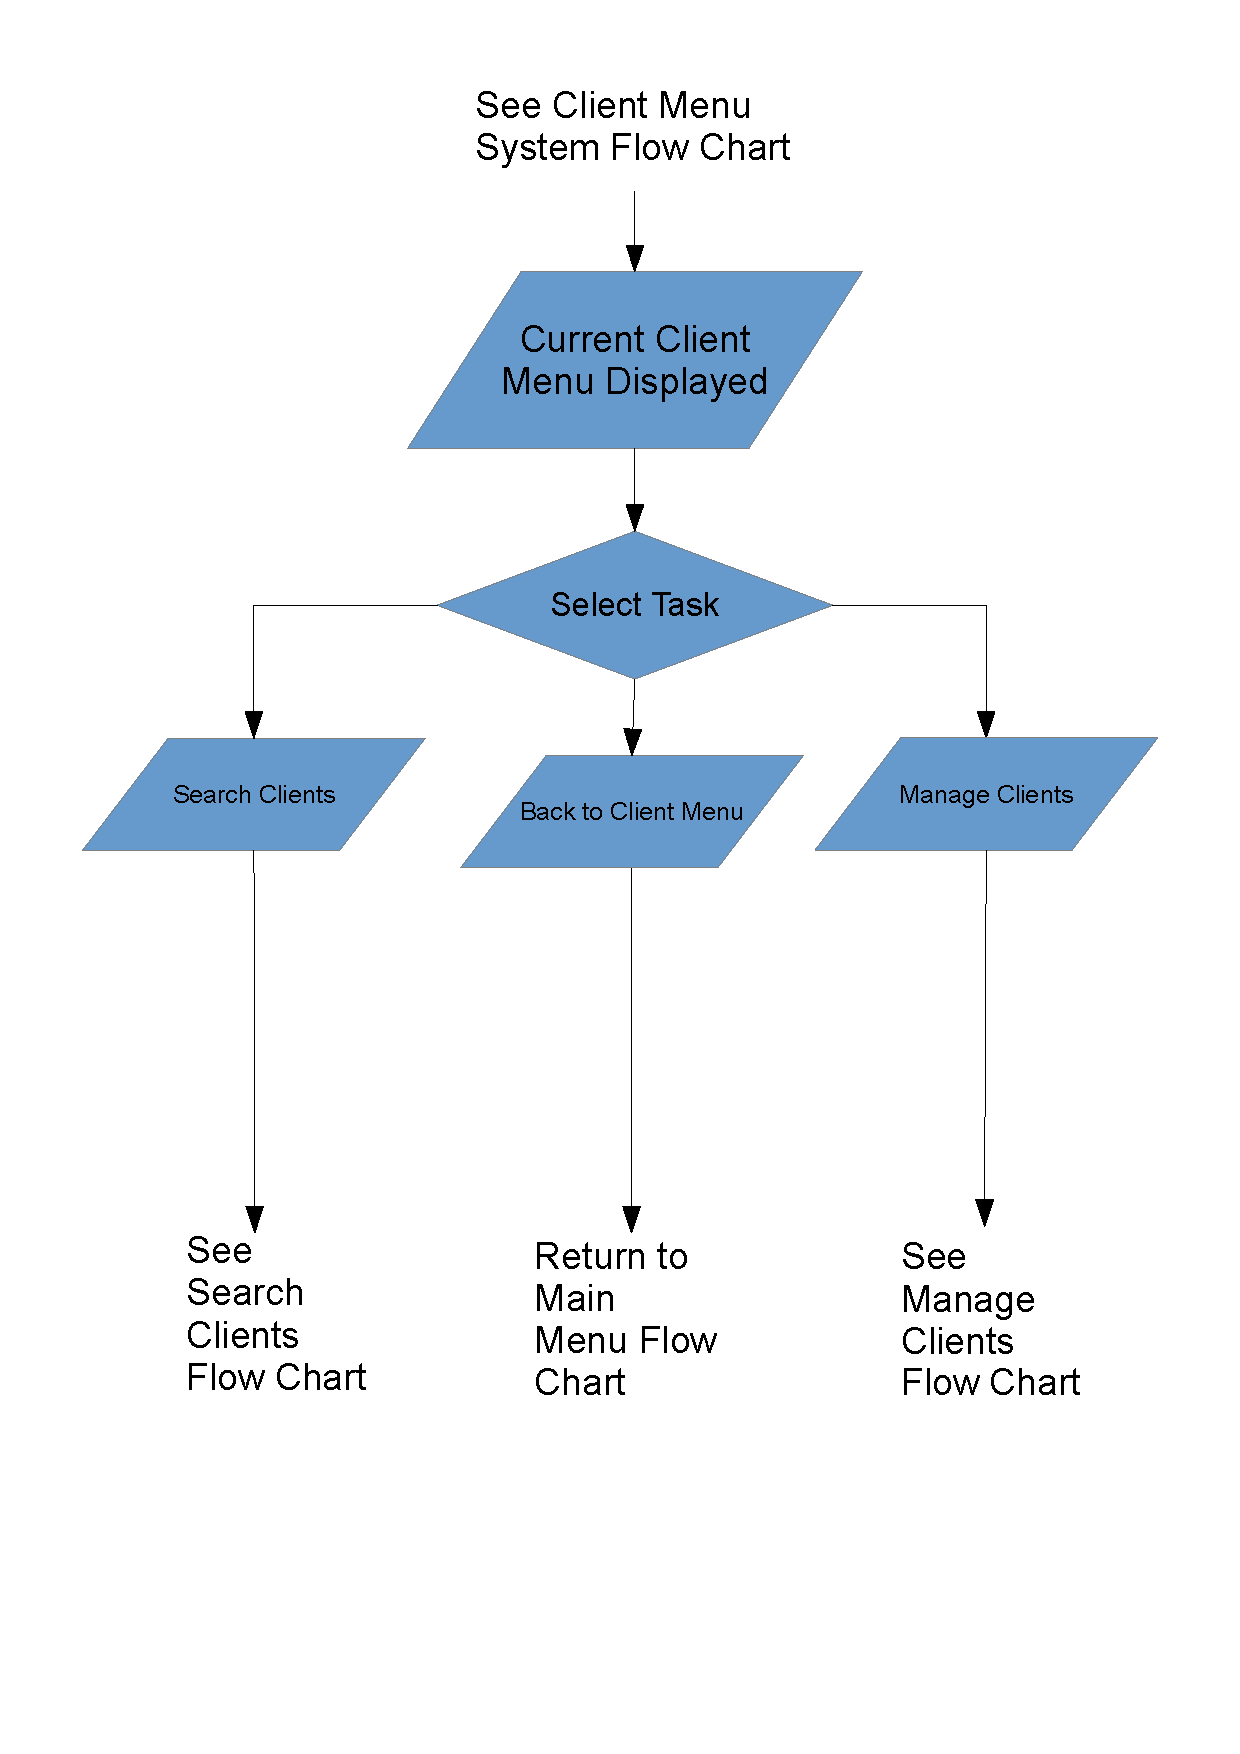
\includegraphics[scale=0.5]{./Design/images/FlowChartCurrentClients.pdf}
    \caption{This is the Current Clients Flow Chart.} 
\label{fig:FlowChartCurrentClients}
\end{figure}

\pagebreak
\textbf{Search Clients Flow Chart}
\begin{flushleft}
Below you can see how you will be able to search the clients in the proposed system. You will be able to search via Location or Search Term etc.
\end{flushleft}
\begin{figure}[H]
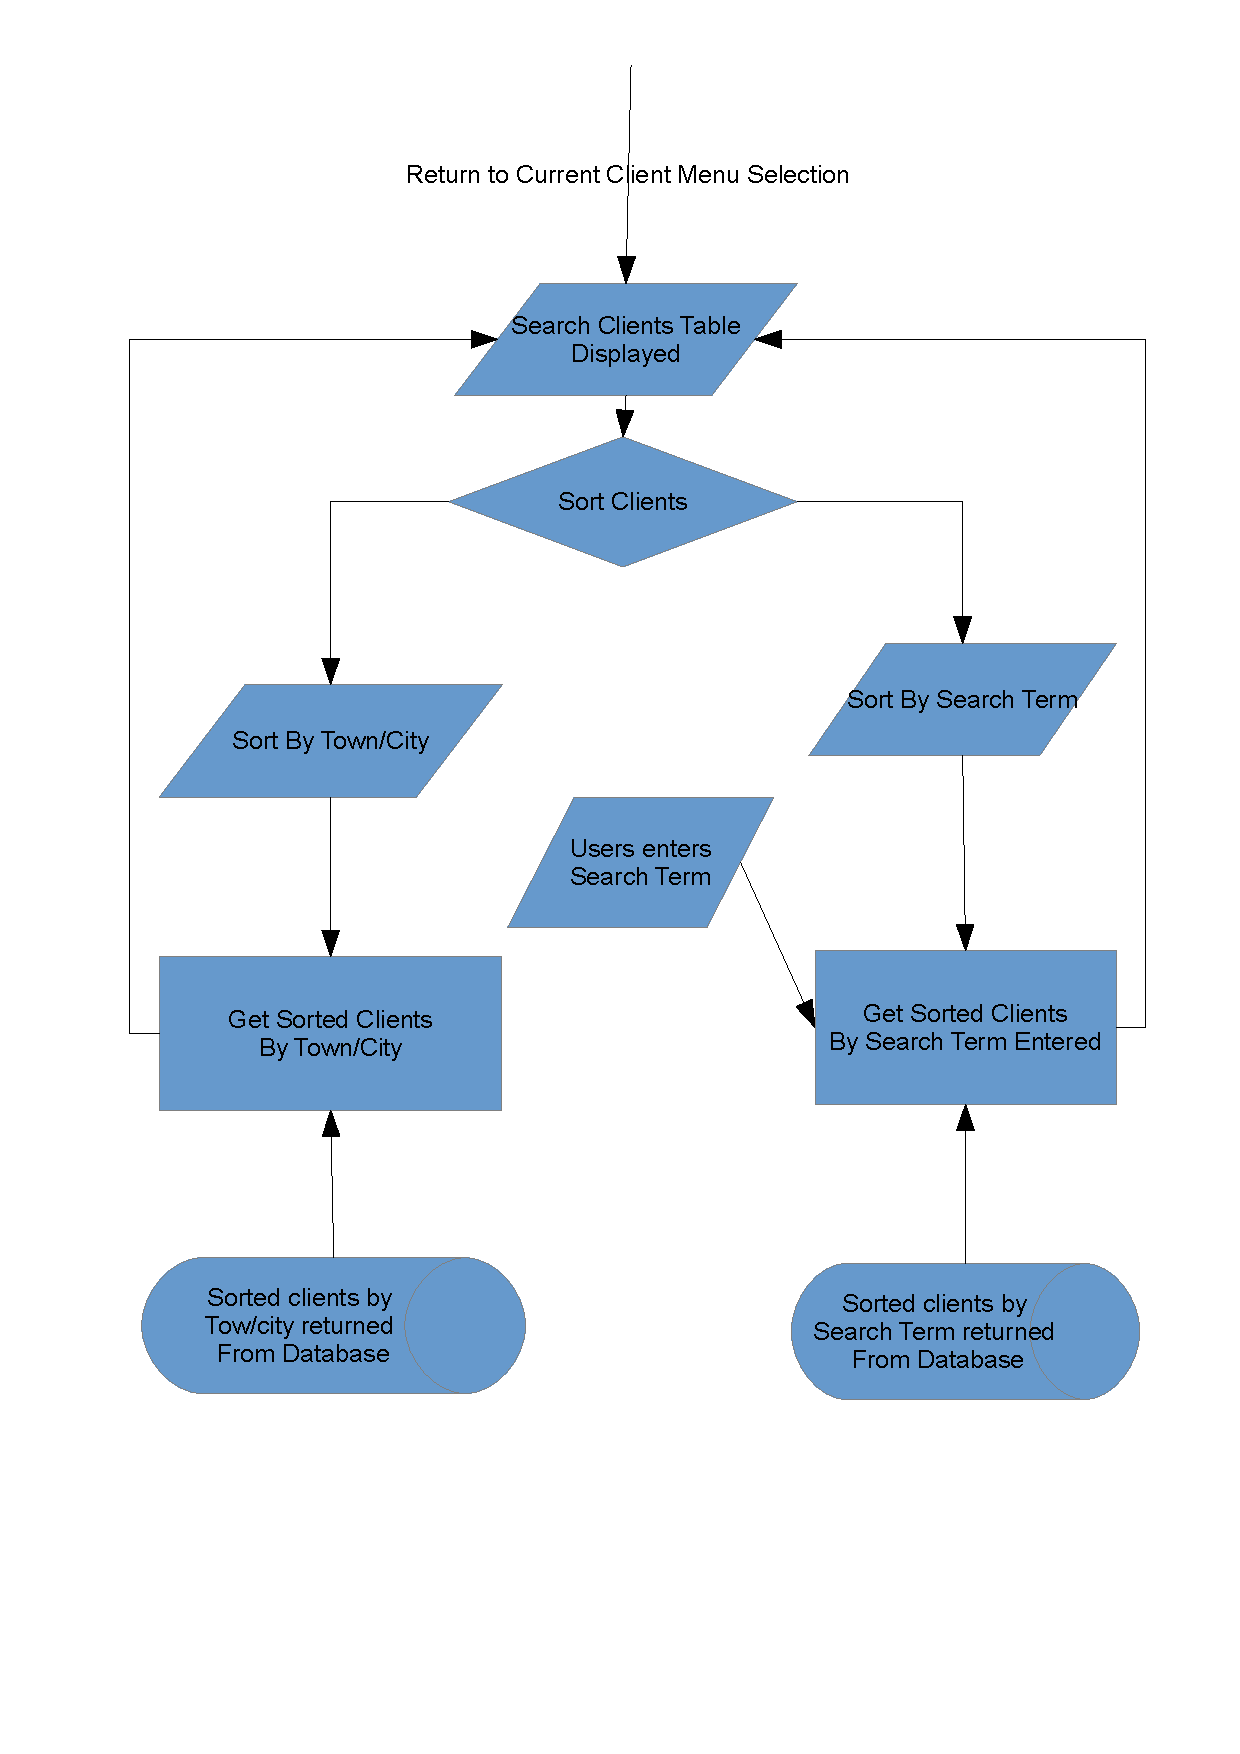
\includegraphics[scale=0.5]{./Design/images/FlowChartSearchClients.pdf}
    \caption{This is the Search Clients Flow Chart.} 
\label{fig:FlowChartSearchClients}
\end{figure}

\pagebreak
\textbf{Manage Clients Flow Chart}
\begin{flushleft}
Below is the manage clients flow chart which shows what happens when you click manage clients in the proposed system.
\end{flushleft}

\begin{figure}[H]
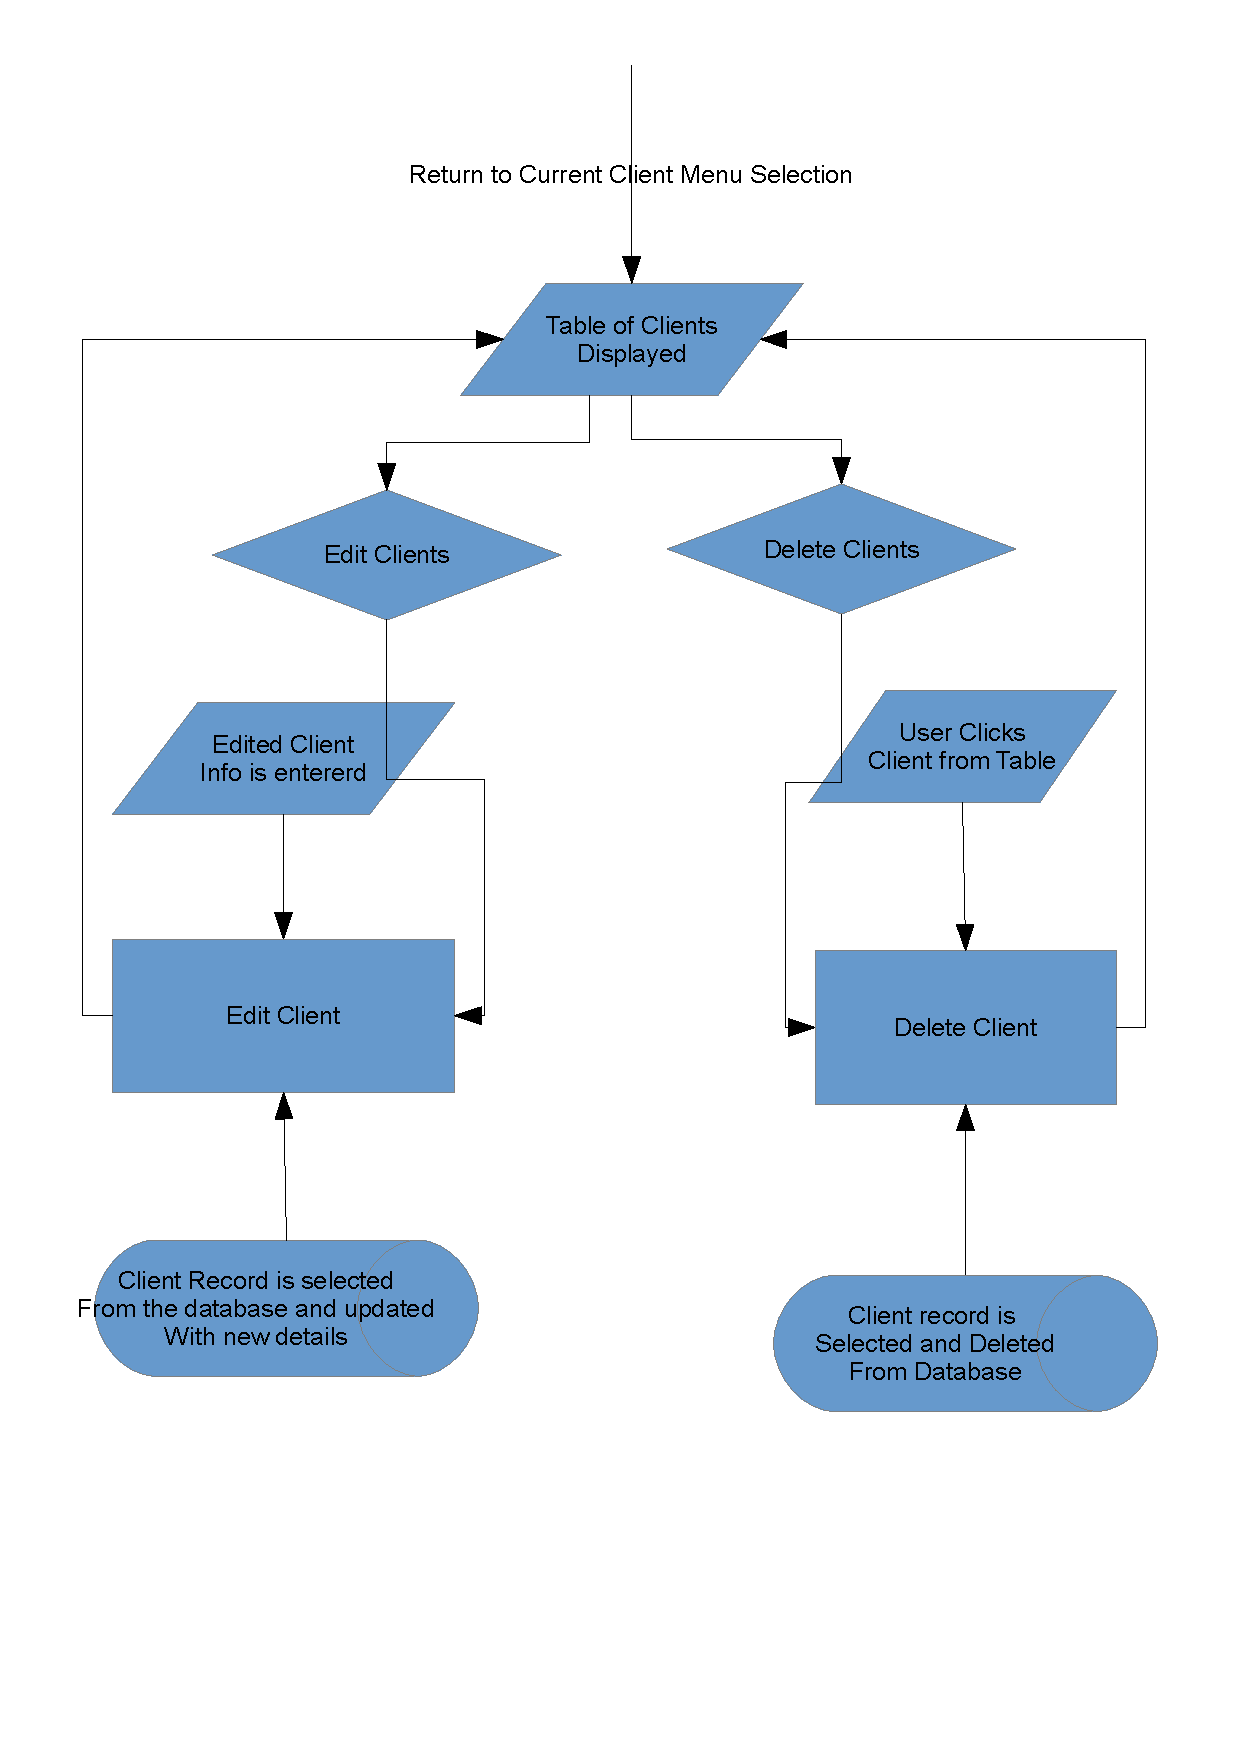
\includegraphics[scale=0.5]{./Design/images/FlowChartManageClients.pdf}
    \caption{This is the Manage Clients Flow Chart.} 
\label{fig:FlowChartSearchClients}
\end{figure}




\pagebreak
\underline{\textbf{Plasterer Flow Charts}}
\par
\begin{flushleft}
The flow charts below are from the plasterer section of the application. They show the options that can be selected for plasterers such as searching,editing and creating new plasterers.
\end{flushleft}

\textbf{Plasterer Menu Flow Chart}
\begin{flushleft}
This is the plasterer menu flow chart showing what users can do in the plasterers section of the application.
\end{flushleft}

\begin{figure}[H]
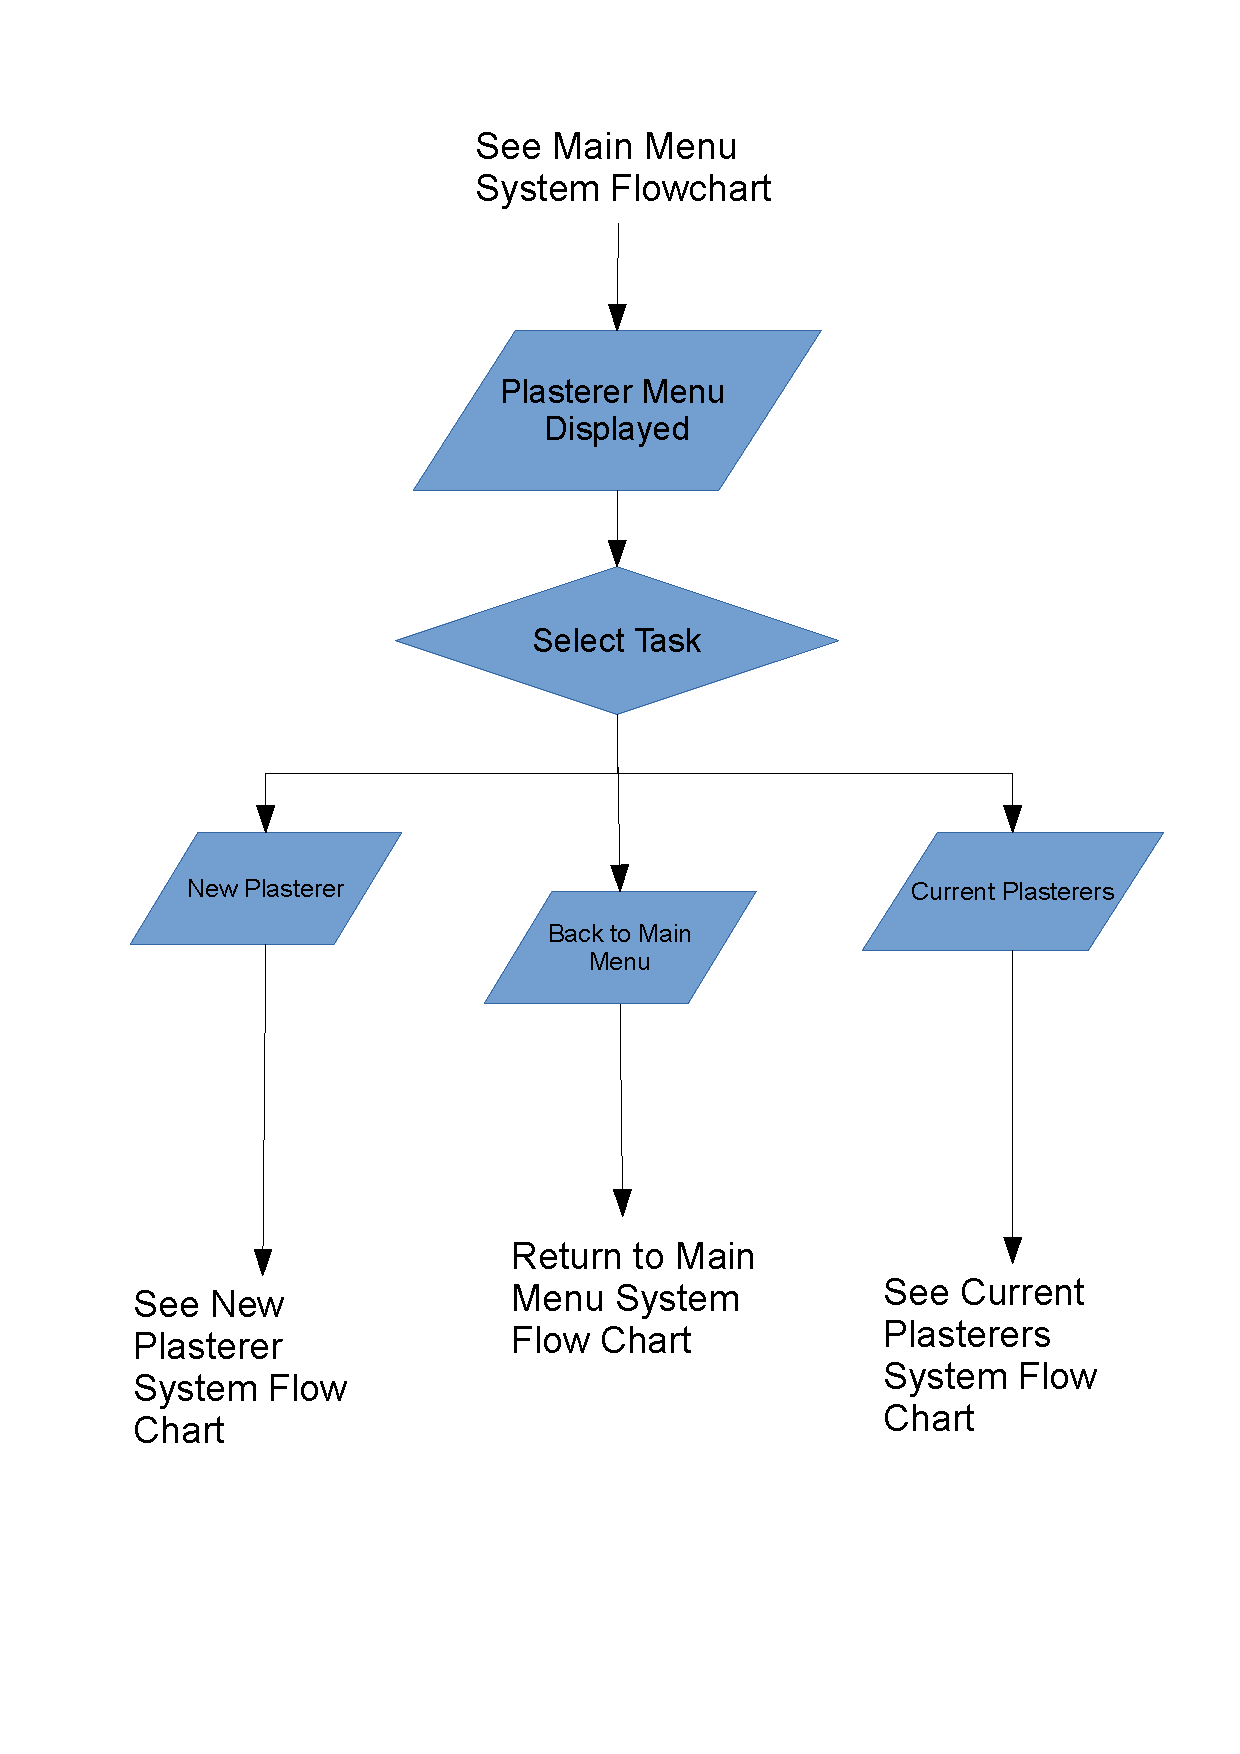
\includegraphics[scale=0.4]{./Design/images/FlowChartPlastererMenu.pdf}
    \caption{This is the Plasterer Menu Flow Chart.} 
\label{fig:FlowChartPlastererMenu}
\end{figure}


\pagebreak
\textbf{Adding a New Plasterer}
\begin{flushleft}
This flow chart shows what happens in the application when you add a new plasterer to the system.
\end{flushleft}

\begin{figure}[H]
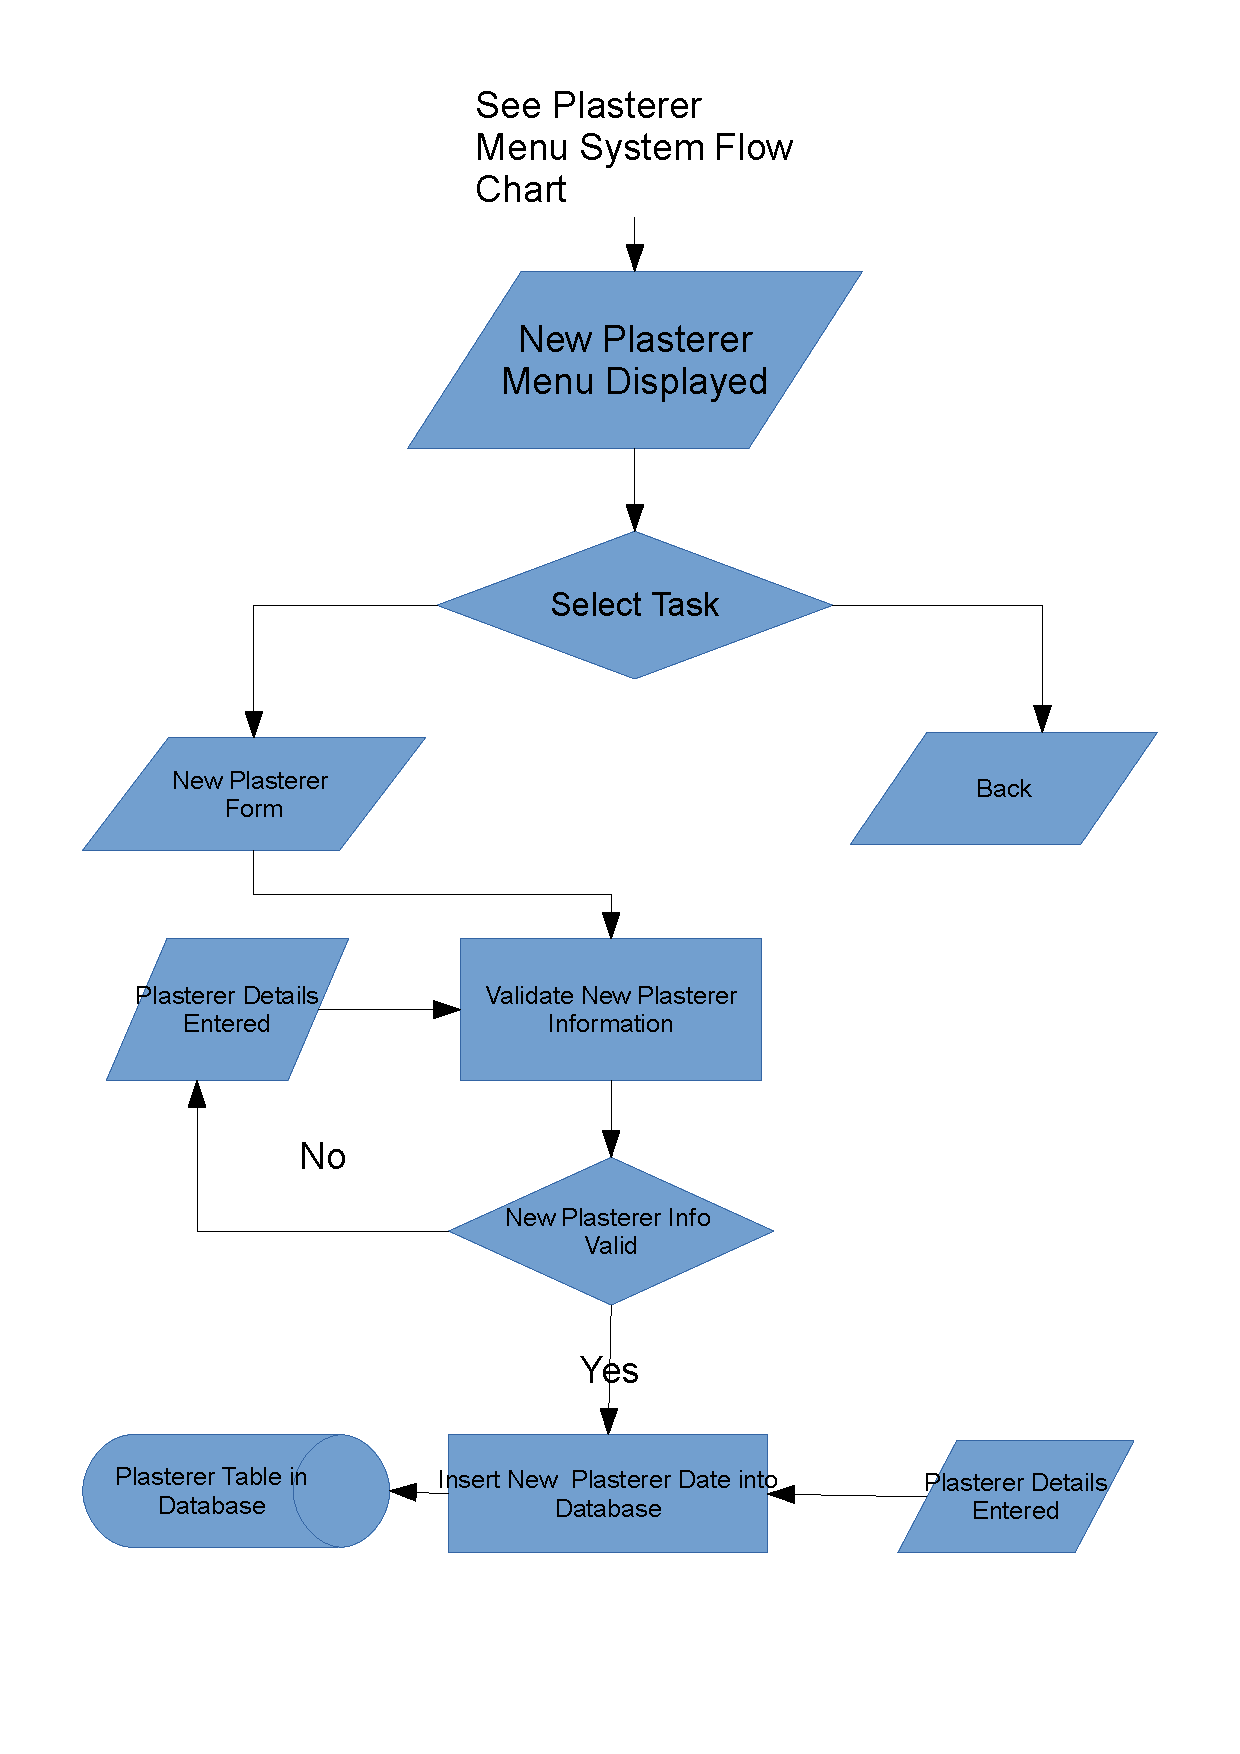
\includegraphics[scale=0.5]{./Design/images/FlowChartNewPlasterer.pdf}
    \caption{This is the New Plasterer Flow Chart.} 
\label{fig:FlowChartNewPlasterer}
\end{figure}


\pagebreak
\textbf{Current Plasterers}
\begin{flushleft}
This flow chart shows the current plasterers options from within the application.
\end{flushleft}

\begin{figure}[H]
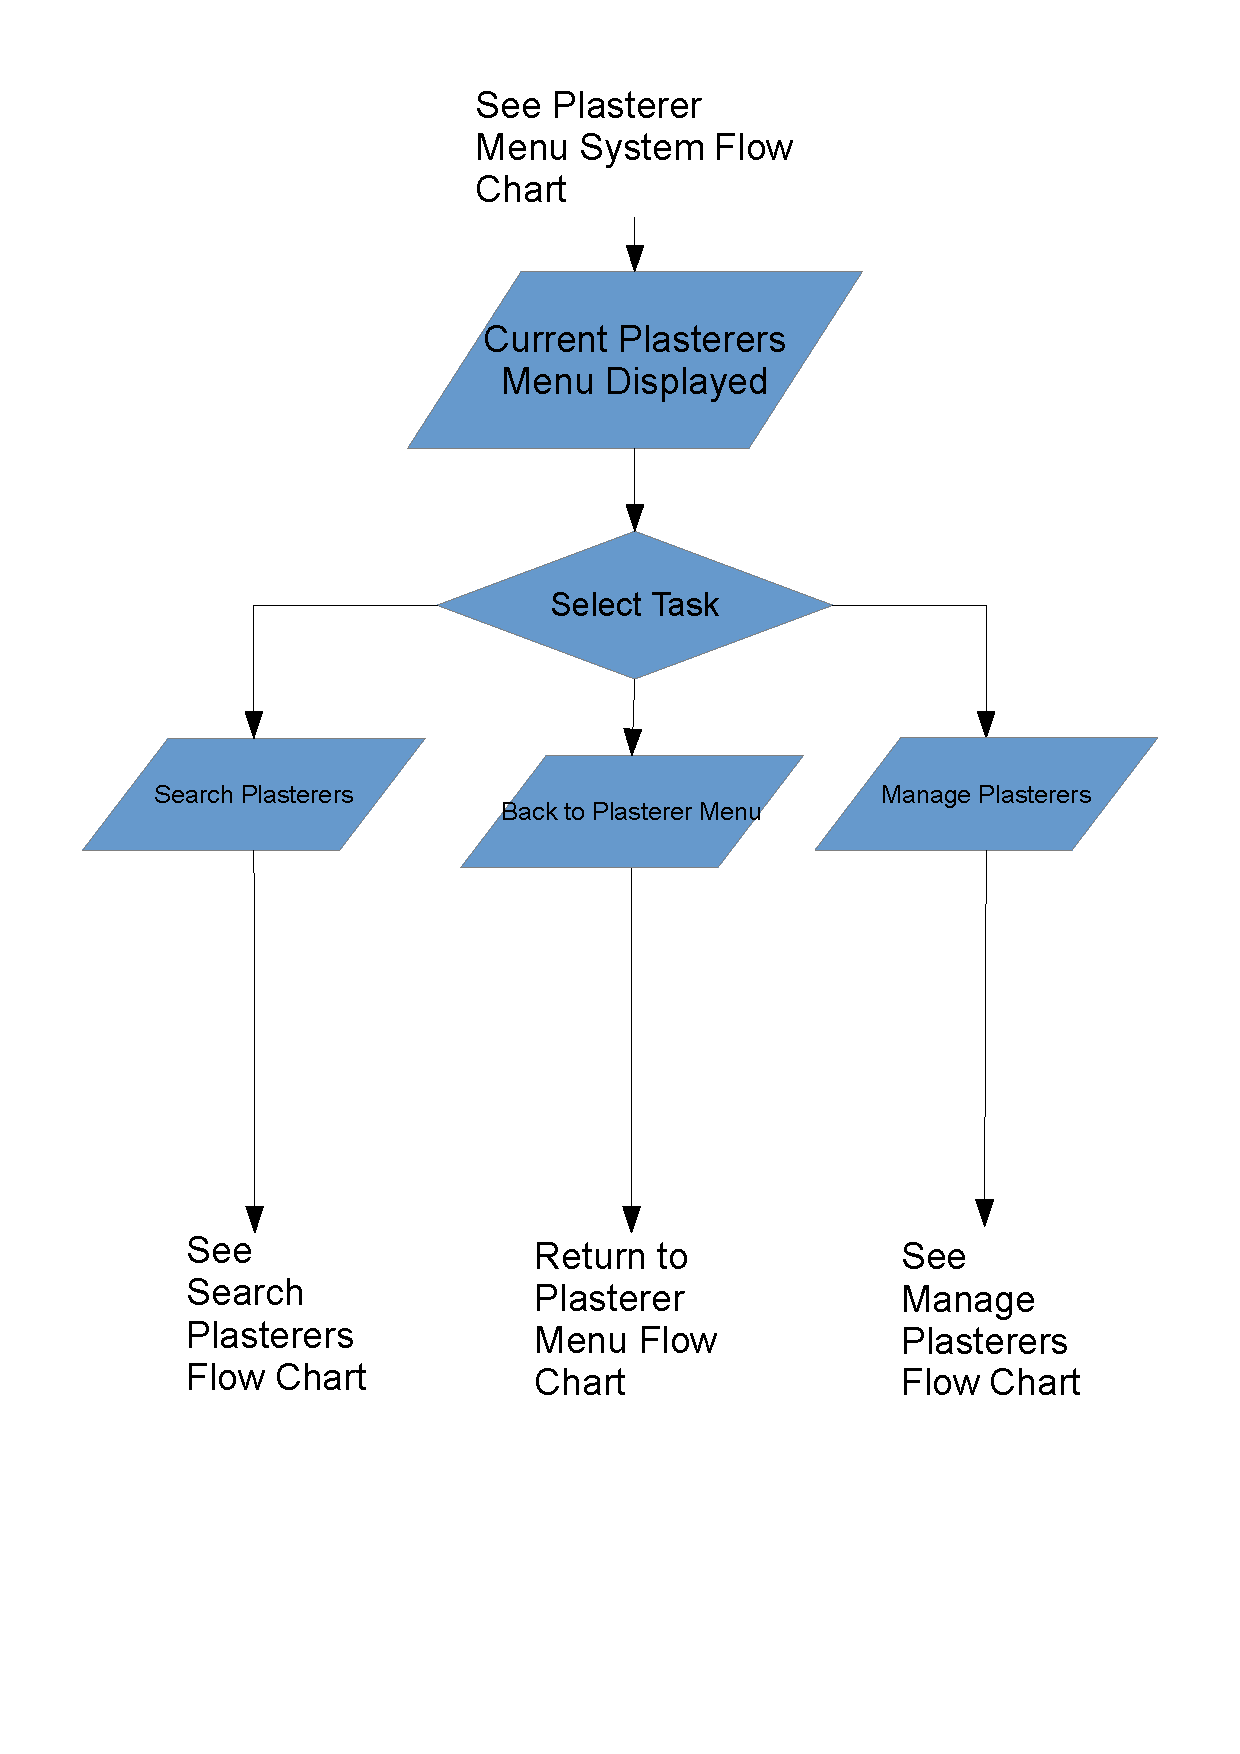
\includegraphics[scale=0.5]{./Design/images/FlowChartCurrentPlasterers.pdf}
    \caption{This is the Current Plasterers Flow Chart.} 
\label{fig:FlowChartCurrentPlasterers}
\end{figure}


\pagebreak
\textbf{Manage Plasterers}
\begin{flushleft}
This flow chart shows the manage plasterers window from the proposed application.
\end{flushleft}
\begin{figure}[H]
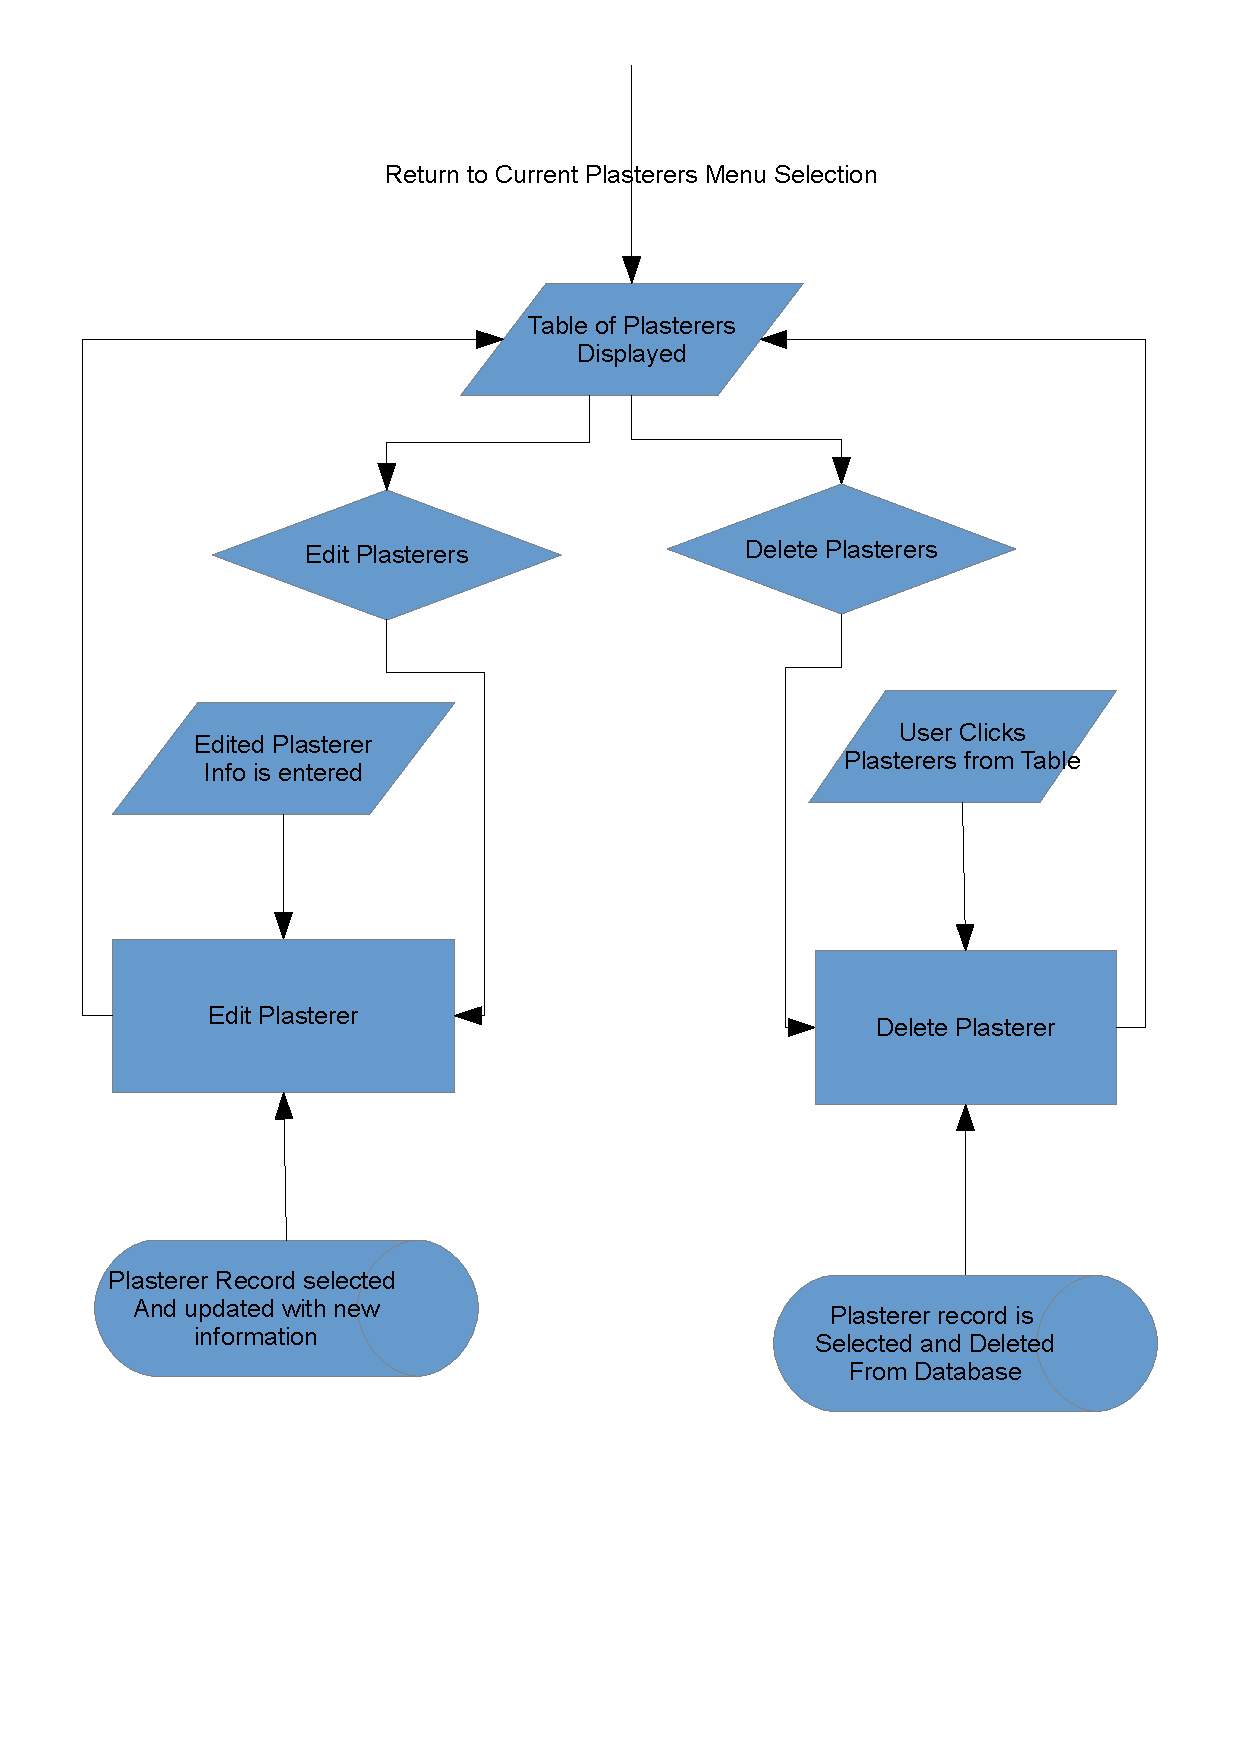
\includegraphics[scale=0.5]{./Design/images/FlowChartManagePlasterers.pdf}
    \caption{This is the Manage Plasterers Flow Chart.} 
\label{fig:FlowChartManagePlasterers}
\end{figure}

\pagebreak
\textbf{Search Plasterers}
\begin{flushleft}
This flow chart shows the search plasterers feature of the proposed application. It lets the user search the plasterers for specific records.
\end{flushleft}
\begin{figure}[H]
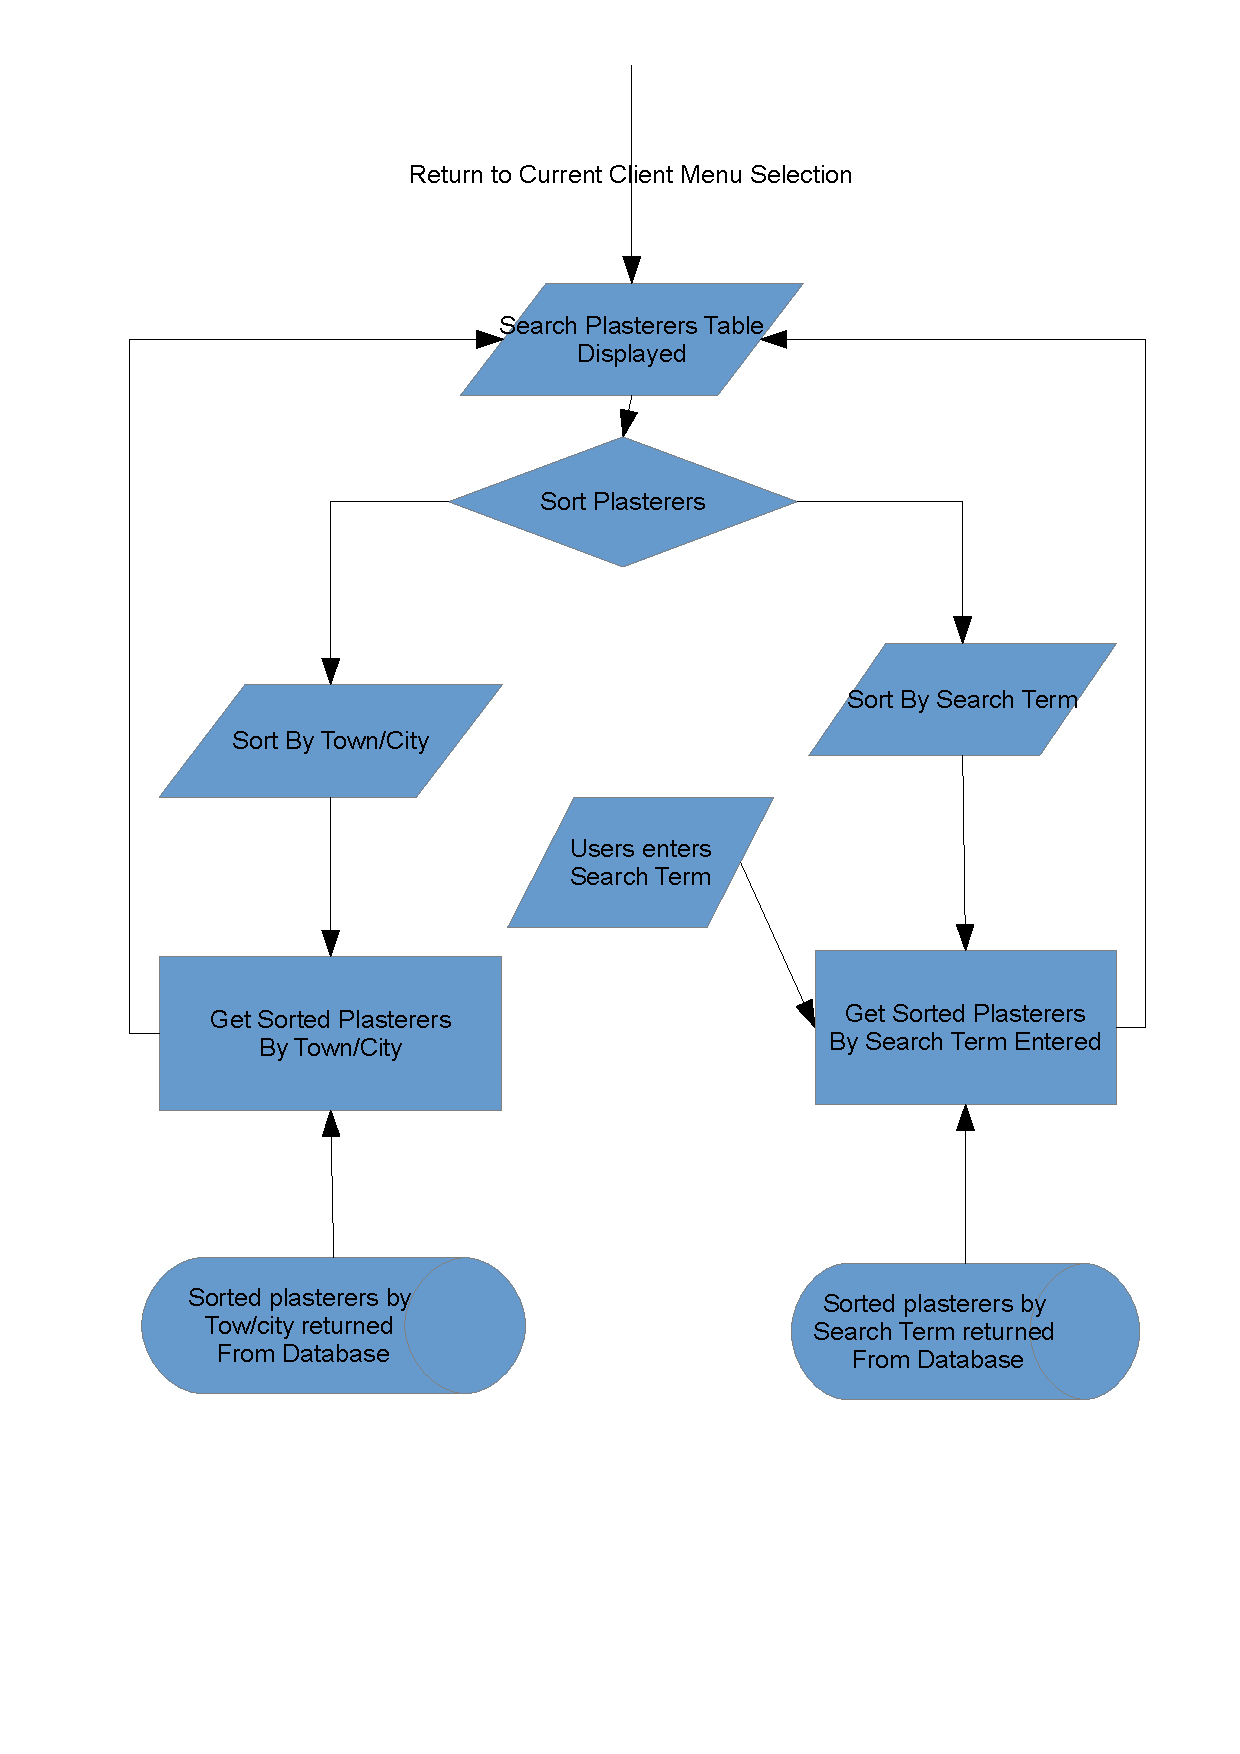
\includegraphics[scale=0.5]{./Design/images/FlowChartSearchPlasterers.pdf}
    \caption{This is the Search Plasterers Flow Chart.} 
\label{fig:FlowChartSearchPlasterers}
\end{figure}



\pagebreak
\underline{\textbf{Jobs Flow Charts}}
\begin{flushleft}
The flow charts below are from the jobs section of the application.
\end{flushleft}
\textbf{Job Menu Flow Chart}
\begin{flushleft}
This flow chart shows the selection choice at the job menu section of the application.
\end{flushleft}
\begin{figure}[H]
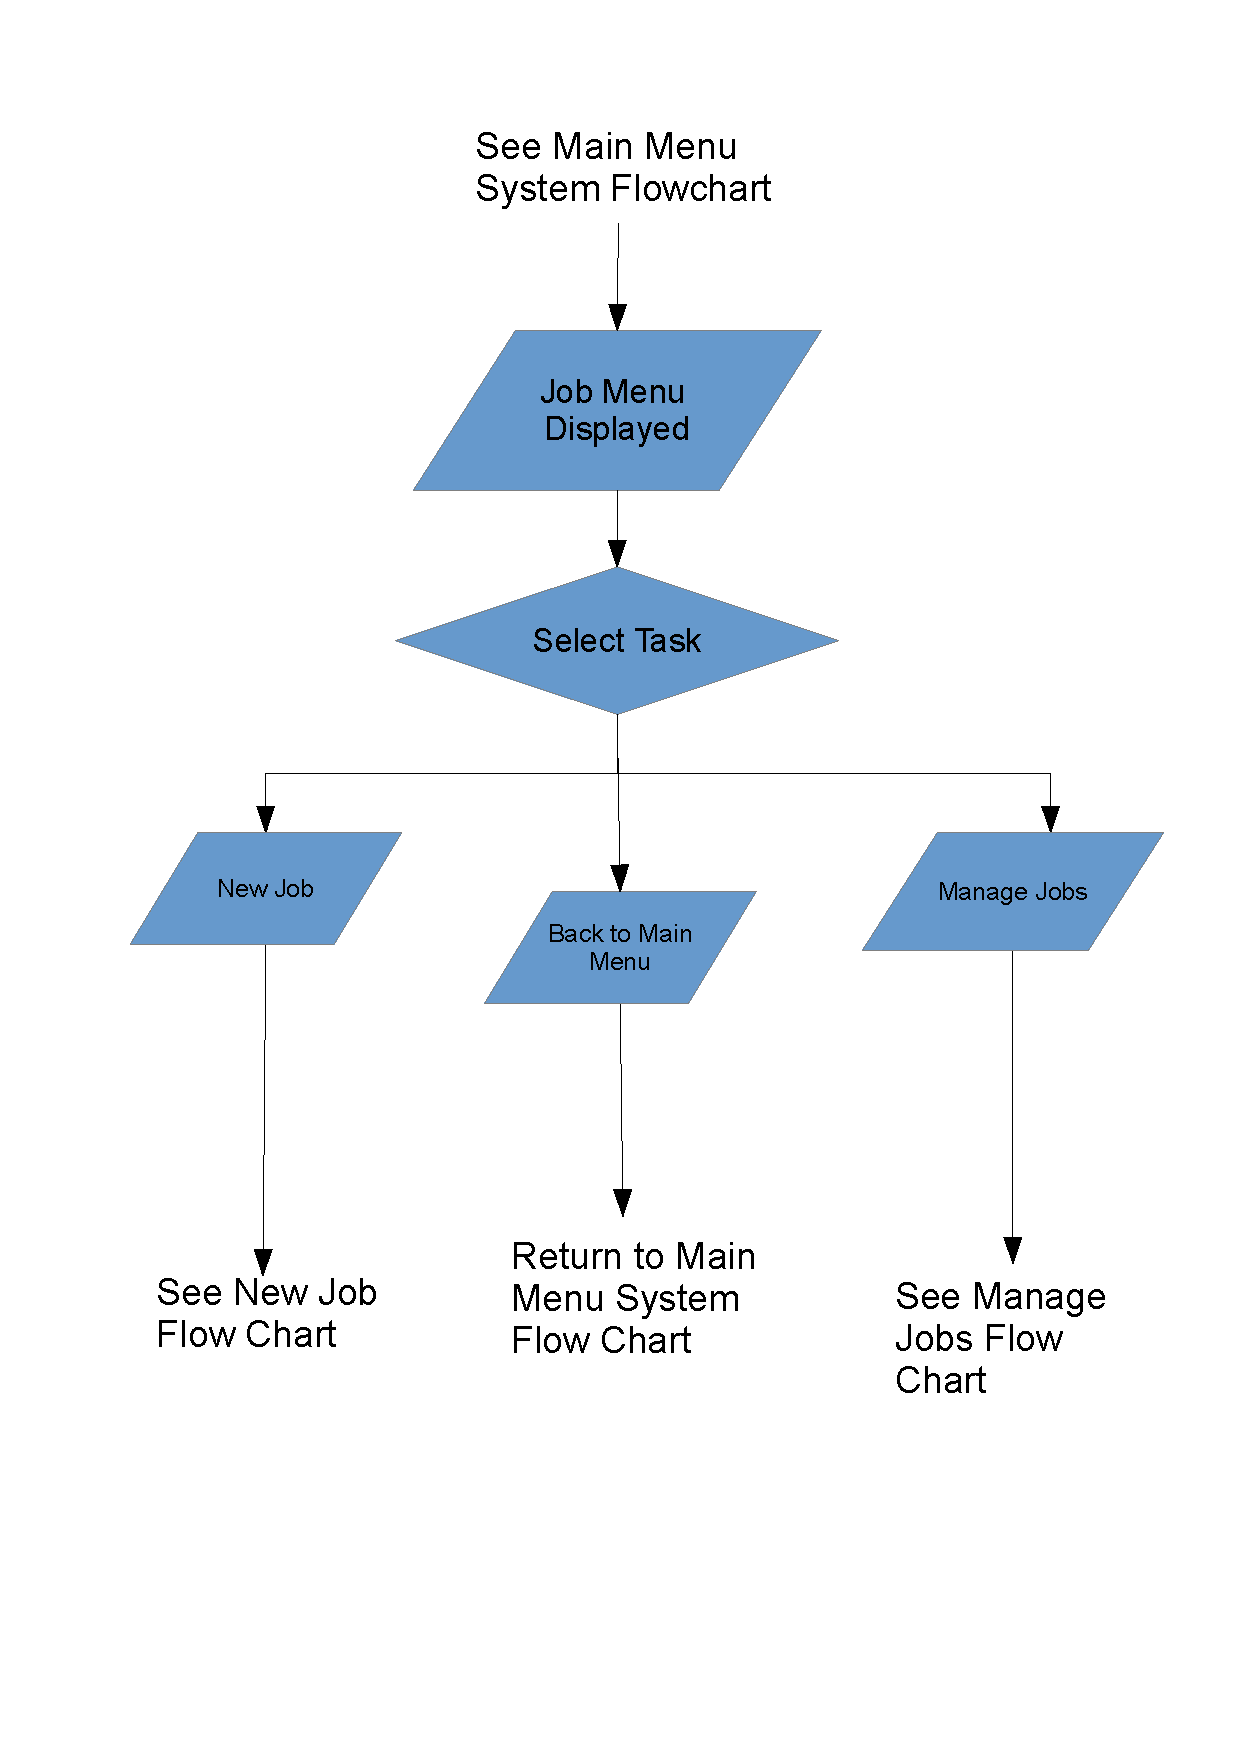
\includegraphics[scale=0.5]{./Design/images/FlowChartJobMenu.pdf}
    \caption{This is the Job Menu Flow Chart.} 
\label{fig:FlowChartJobMenu}
\end{figure}

\pagebreak
\textbf{New Job Flow Chart}
\begin{flushleft}
This flow chart shows what happens in the application when the users adds a new job.
\end{flushleft}
\begin{figure}[H]
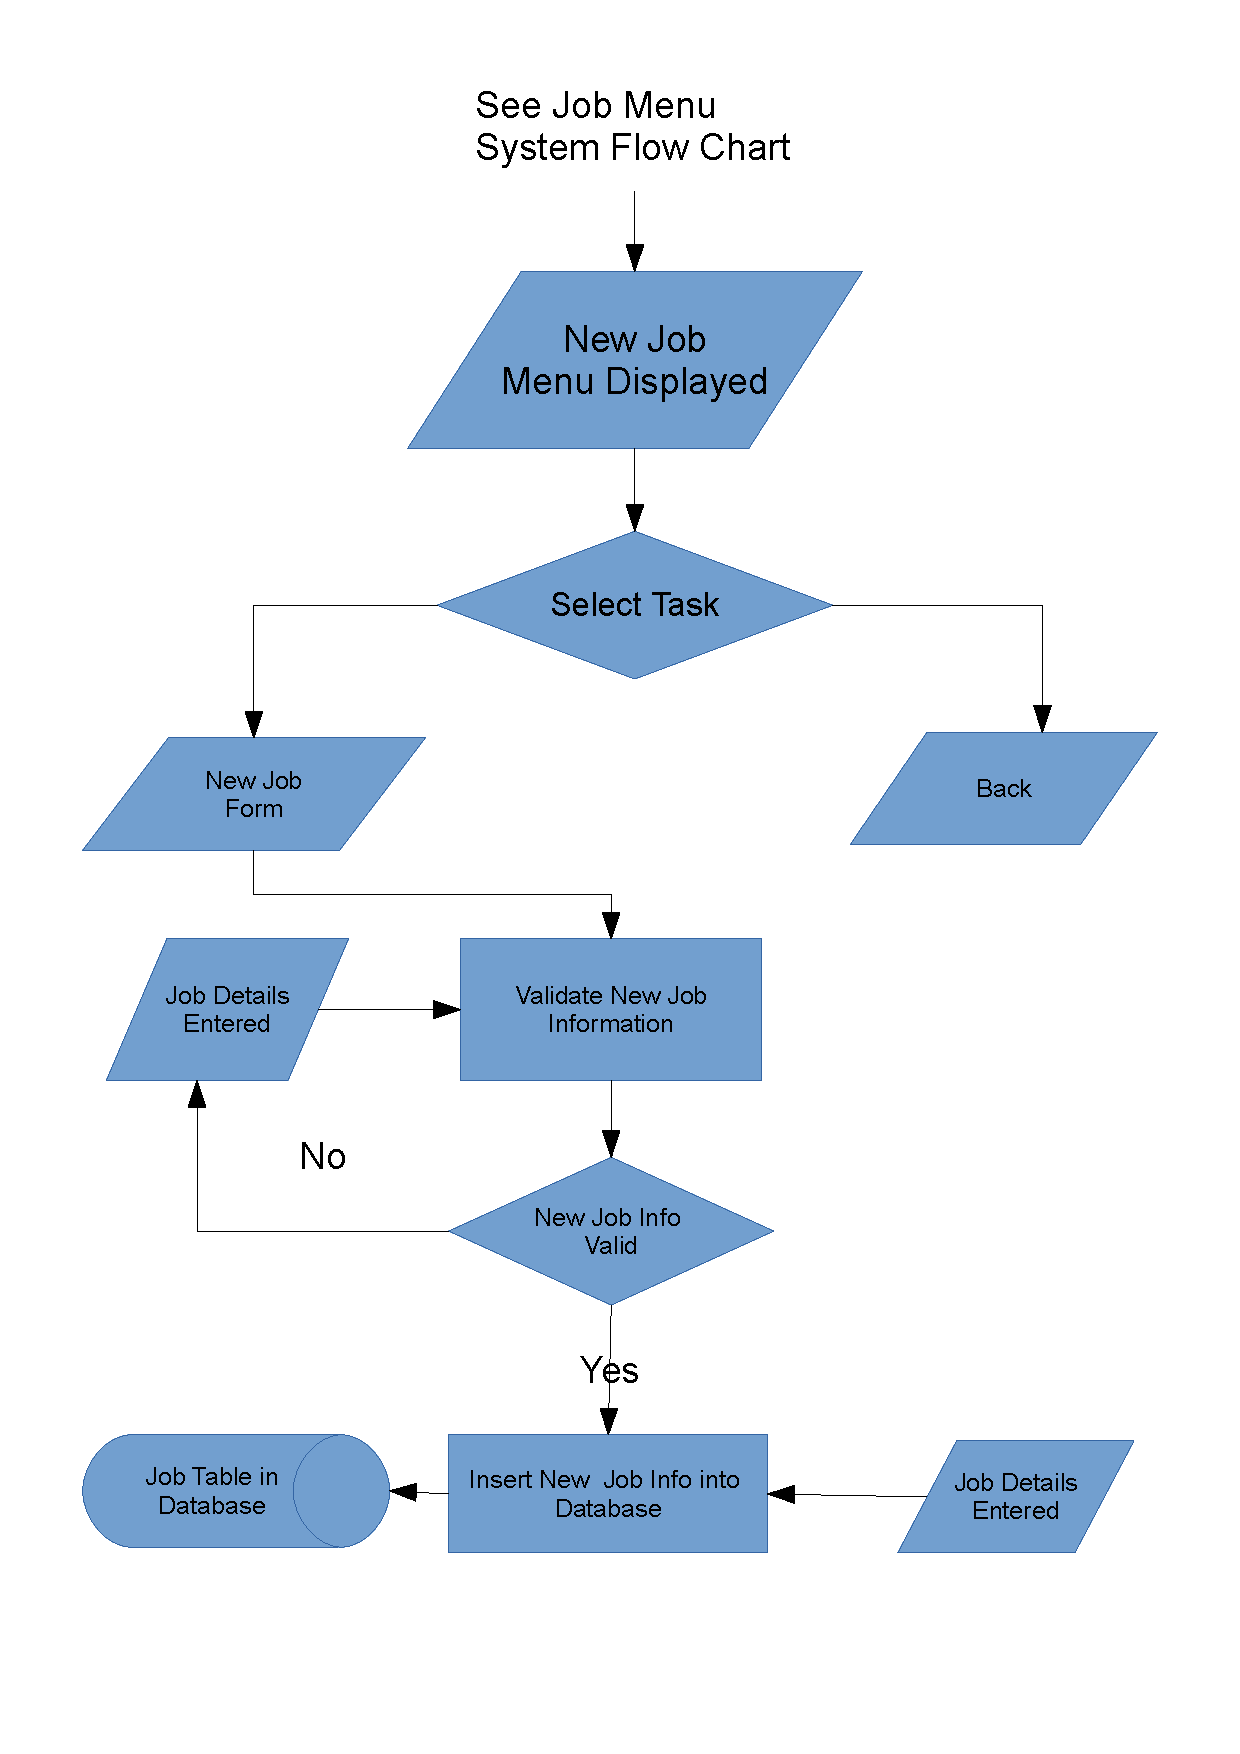
\includegraphics[scale=0.5]{./Design/images/FlowChartNewJob.pdf}
    \caption{This is the New Job Flow Chart.} 
\label{fig:FlowChartNewJob}
\end{figure}


\pagebreak
\textbf{Manage Jobs Flow Chart}
\begin{flushleft}
This shows the manage jobs section of the application.
\end{flushleft}
\begin{figure}[H]
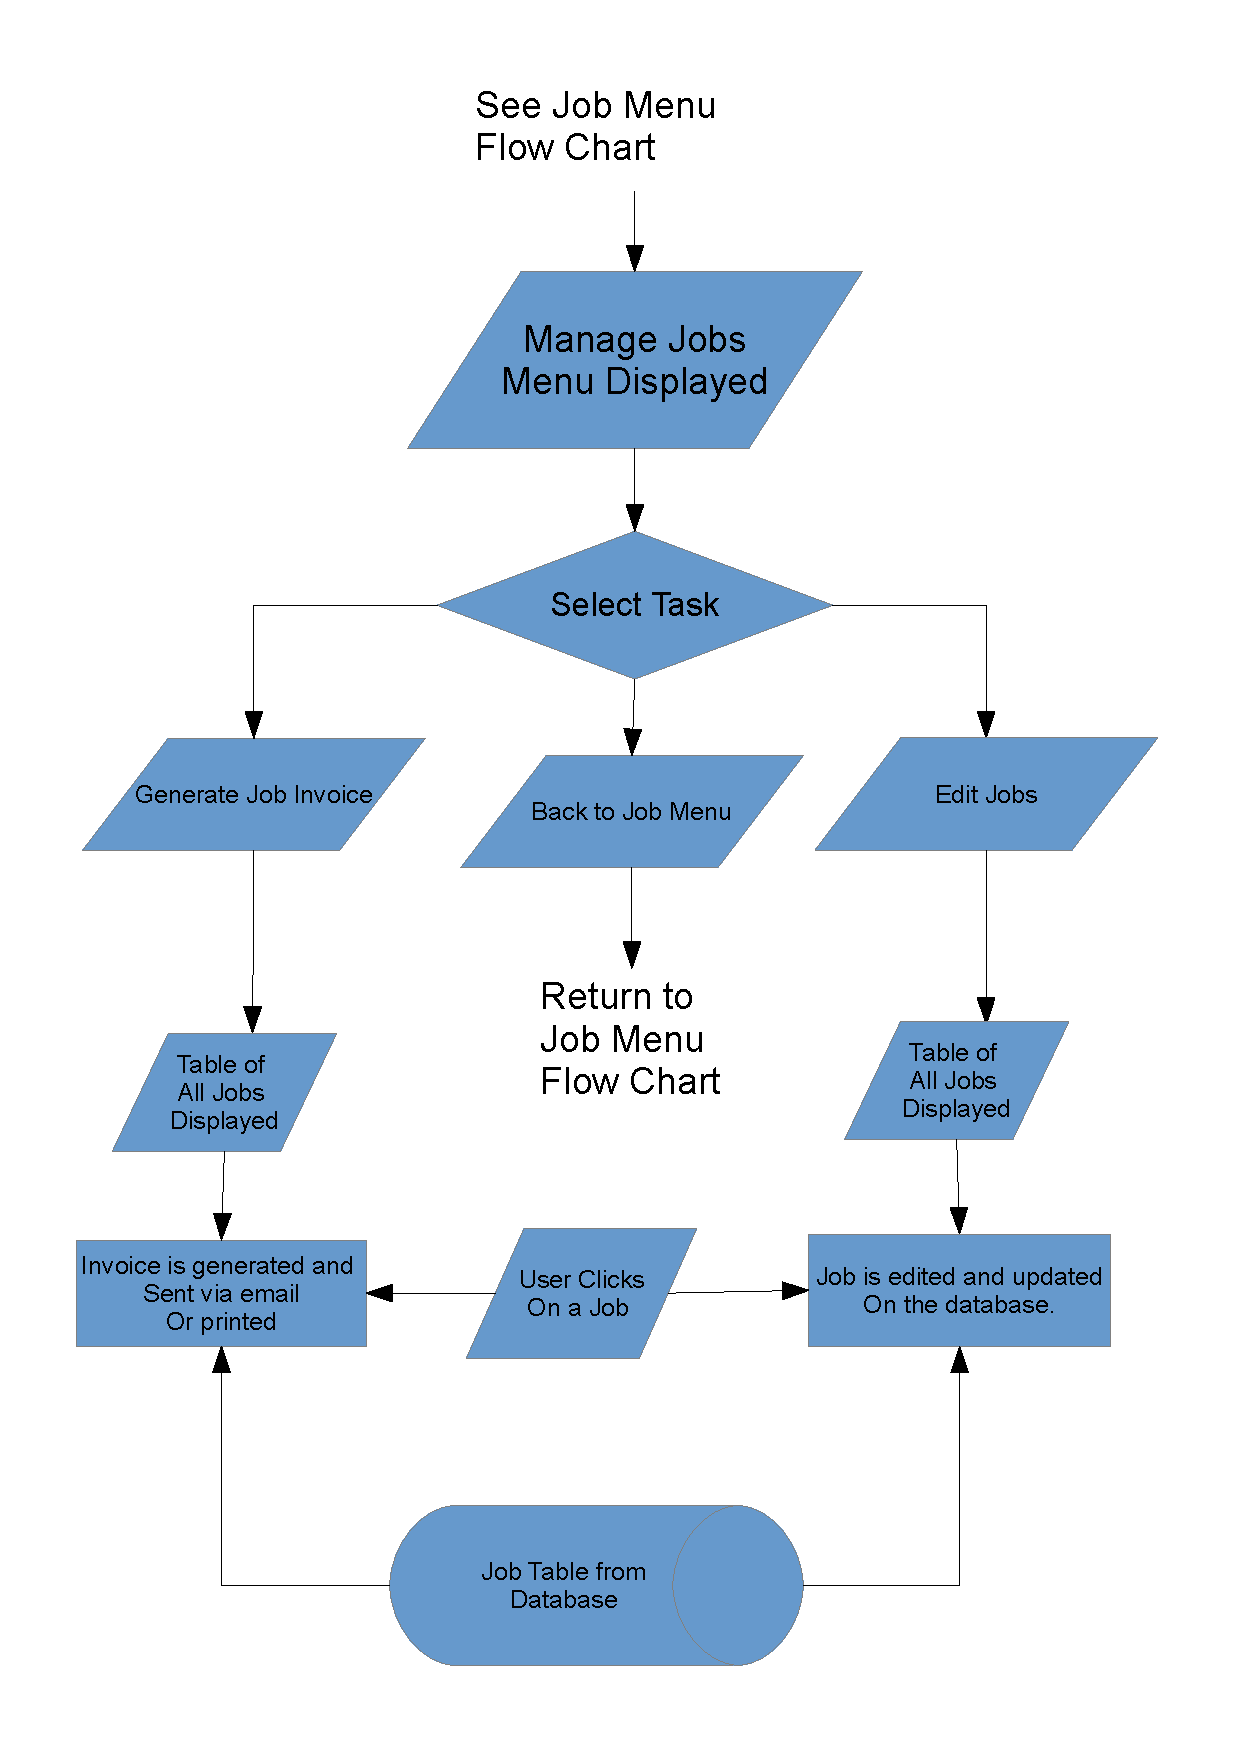
\includegraphics[scale=0.5]{./Design/images/FlowChartManageJobs.pdf}
    \caption{This is the Manage Jobs Flow Chart.} 
\label{fig:FlowChartManageJobs}
\end{figure}



\section{User Interface Designs}
\textbf{Main Menu To Clients Menu UI}
\begin{flushleft}
This shows what the user interface will look and behave like when the clients button is clicked.
\end{flushleft}
\begin{figure}[H]
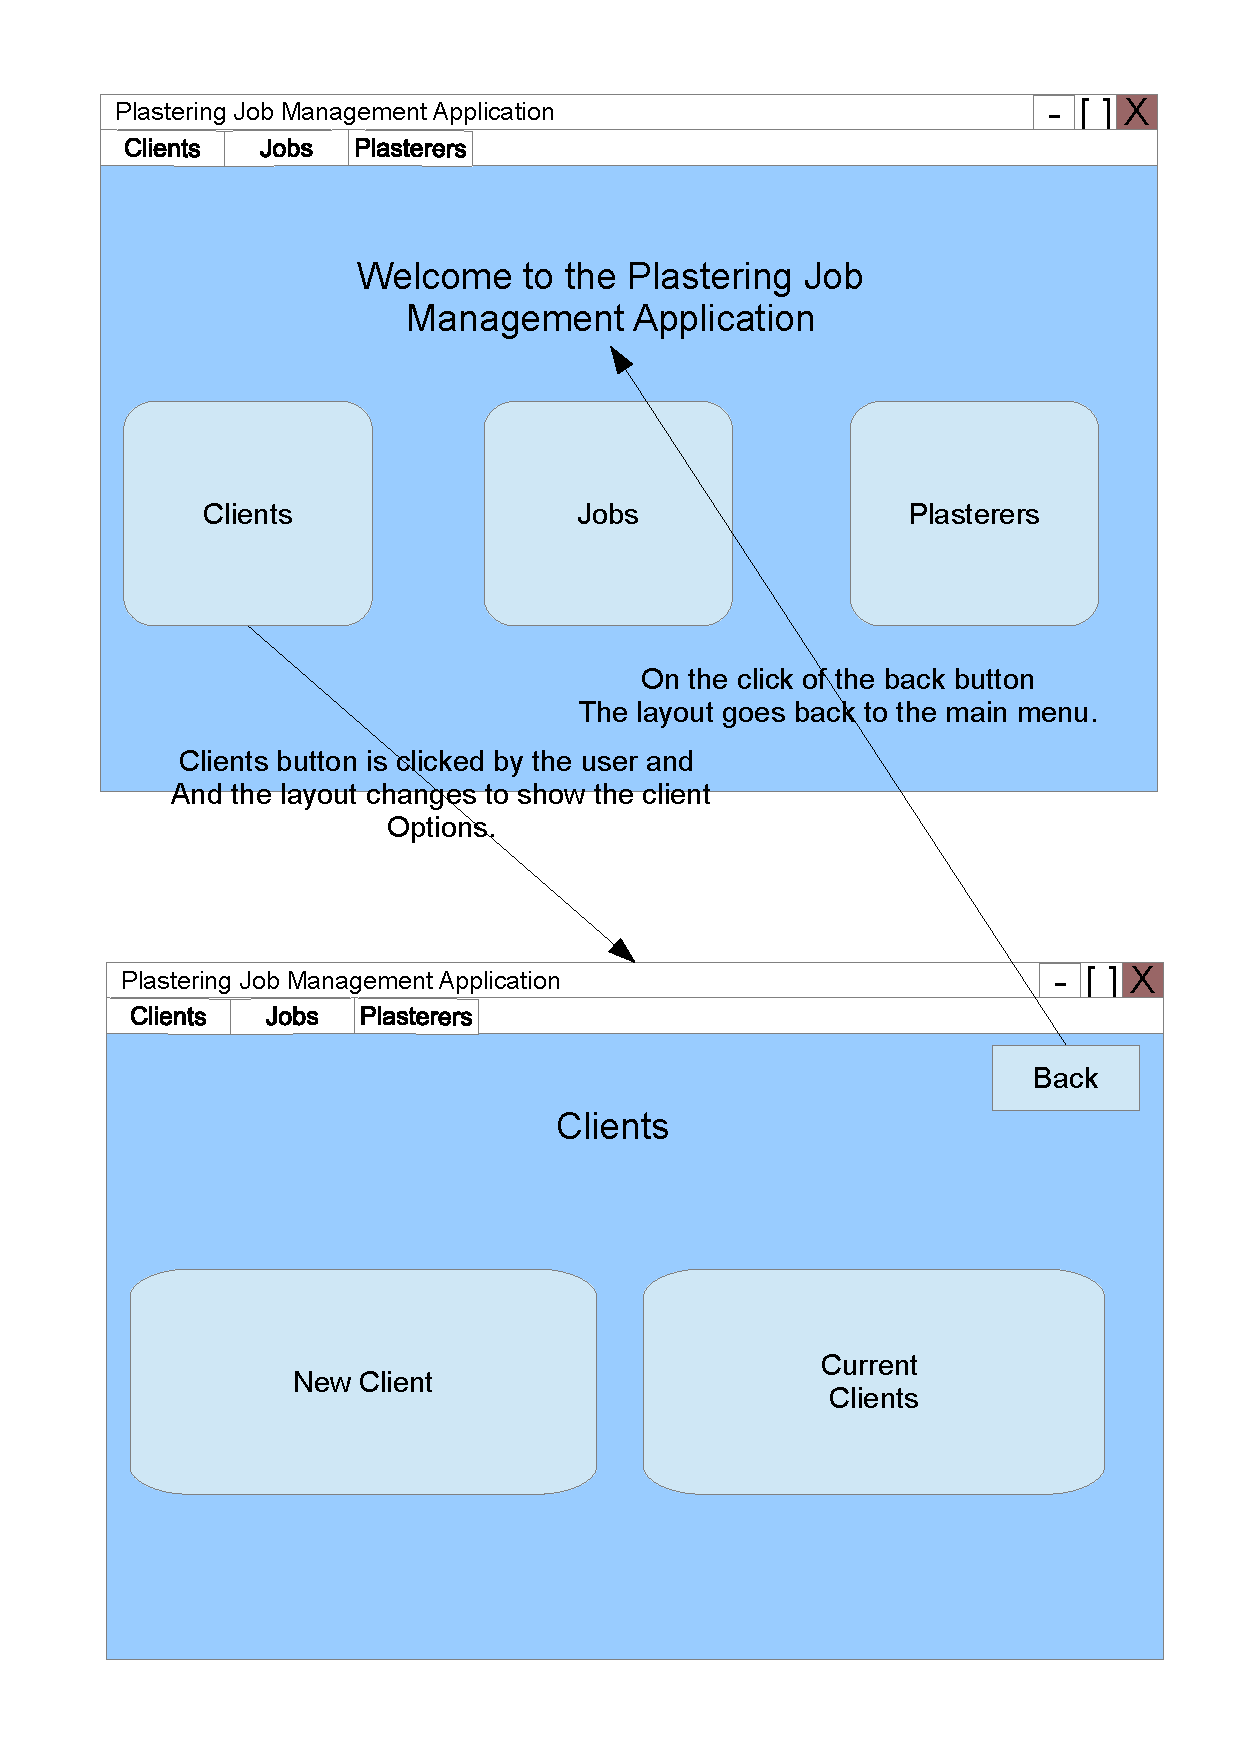
\includegraphics[scale=0.5]{./Design/images/UI-ClientsMenu.pdf}
    \caption{This is the Clients Menu User Interface.} 
\label{fig:FlowChartClientsMenu}
\end{figure}

\textbf{Clients Menu to New Client UI}
\begin{flushleft}
This User Interface diagram shows what happens in the proposed system when the users adds a new client.
\end{flushleft}
\begin{figure}[H]
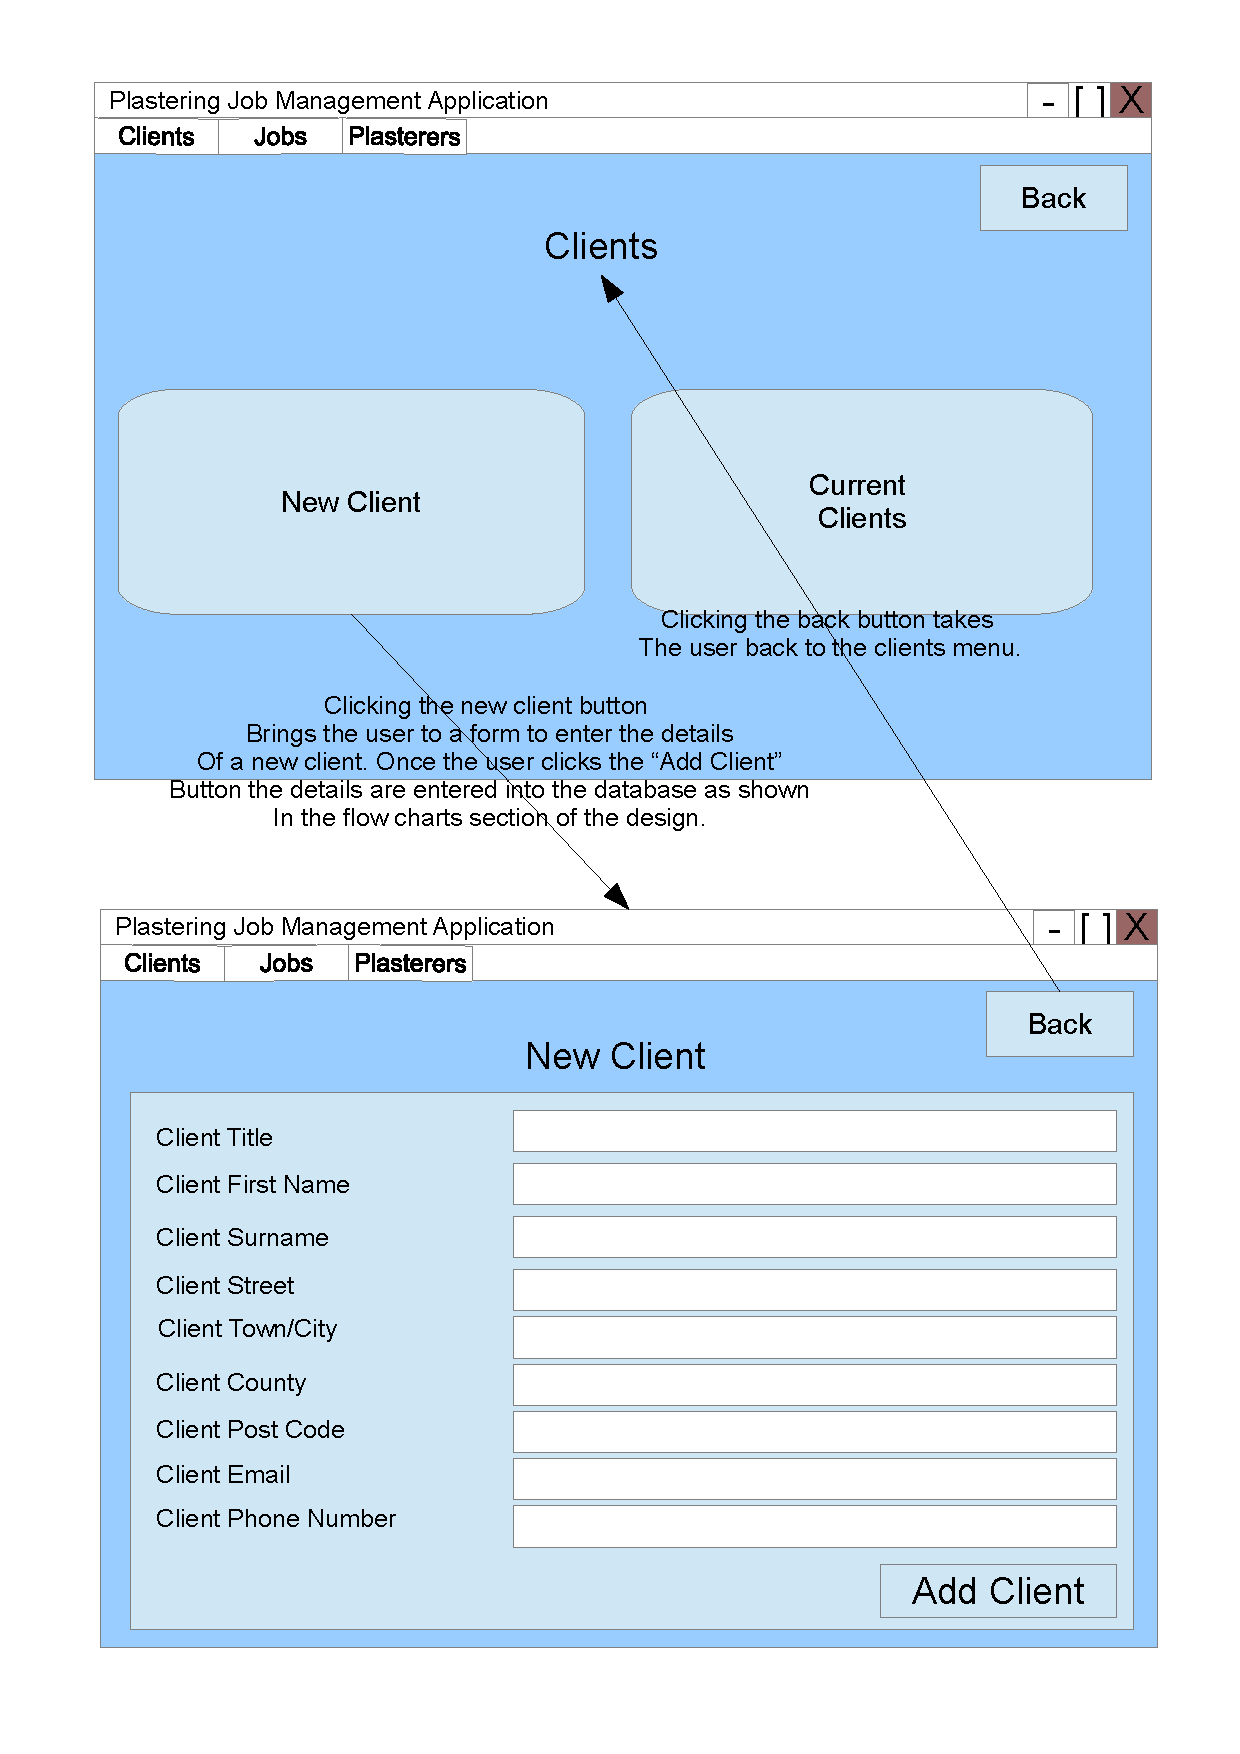
\includegraphics[scale=0.5]{./Design/images/UI-NewClient.pdf}
    \caption{This is the New Client User Interface.} 
\label{fig:FlowChartNewClient}
\end{figure}

\section{Hardware Specification}

\section{Program Structure}

\subsection{Top-down design structure charts}




\subsection{Algorithms in pseudo-code for each data transformation process}

\pagebreak
\subsection{Object Diagrams}
\begin{flushleft}
This Diagram shows the relationship between the objects in the system.
\end{flushleft}
\begin{figure}[H]
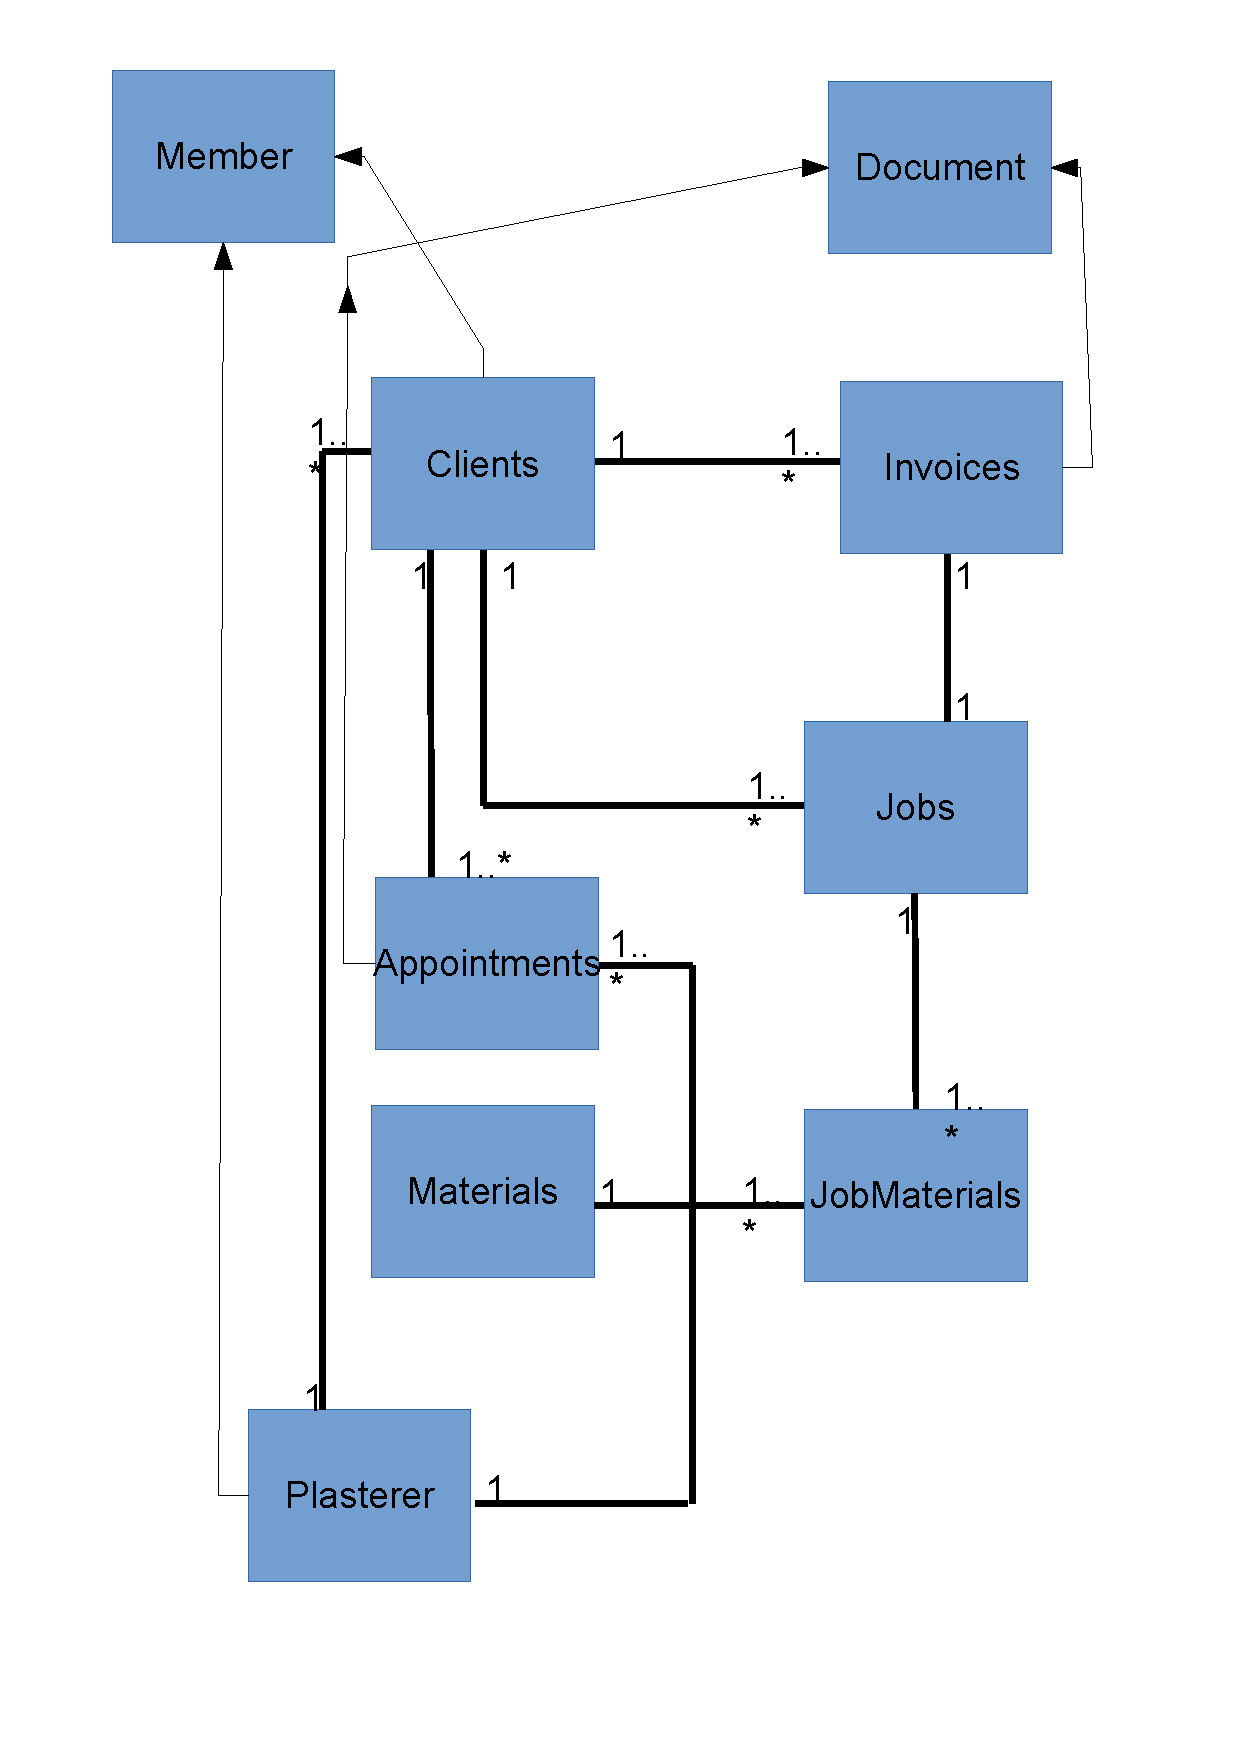
\includegraphics[scale=0.5]{./Design/images/ObjectDiagram.pdf}
    \caption{Object Relationships} 
\label{fig:ObjectDiagram}
\end{figure}



\pagebreak
\subsection{Class Definitions}

\begin{flushleft}
\textbf{Key:}
\begin{tabular}{|p{4cm}|}
	\hline
	Label \\ \hline
	Attributes \\ \hline	
	Behavious \\ \hline
\end{tabular}


\end{flushleft}

\begin{tabular}{|p{4cm}|}
	\hline
	\textbf{Member} \\ \hline
	MemberID \\
	MemberTitle \\
	MembeFirstName \\
	MemberSurname \\
	MemberAddrLine1 \\
	MemberAddrLine2 \\
	MemberAddrLine3 \\
	MemberAddrLine4 \\
	MemberEmail \\
	MemberPhoneNumber \\ \hline	
		AddMemberTitle \\
		AddMemberFirstName \\
		AddMemberSurname \\
		AddMemberAddrLine1 \\
		AddMemberAddrLine2 \\
		AddMemberAddrLine3 \\
		AddMemberAddrLine4 \\
		AddMemberEmail \\
		AddMemberPhoneNumber \\ 
		EditMemberTitle \\
		EditMemberFirstName \\
		EditMemberSurname \\
		EditMemberAddrLine1 \\
		EditMemberAddrLine2 \\
		EditMemberAddrLine3 \\
		EditMemberAddrLine4 \\
		EditMemberEmail \\
		EditMemberPhoneNumber \\ \hline
\end{tabular}

\begin{tabular}{|p{5cm}|}
	\hline
	\textbf{Client:} extends \textbf{Member} \\ \hline
		 \\ \hline
		 \\ \hline
\end{tabular}


\begin{tabular}{|p{5cm}|}
	\hline
	\textbf{Plasterer:} extends \textbf{Member} \\ \hline
		PlastererDailyRate \\ \hline
		AddPlastererDailyRate \\
		EditPlastererDailyRate \\ \hline
\end{tabular}

\begin{tabular}{|p{5cm}|}
	\hline
	\textbf{Job:} \\ \hline
		JobID \\
		ClientID \\
		PlastererID \\
		JobDescription \\
		JobAddrLine1 \\
		JobAddrLine2 \\
		JobAddrLine3 \\
		JobAddrLine4 \\
		JobDaysWorked \\
		JobComplete \\
		JobPaid \\ 
		InvoiceID \\ \hline
		AddJobDescription\\
		AddJobAddrLine1 \\
		AddJobAddrLine2 \\
		AddJobAddrLine3 \\
		AddJobAddrLine4 \\
		AddJobDaysWorked \\
		EditJobComplete \\
		EditJobPaid \\
		EditJobDescription\\
		EditJobAddrLine1 \\
		EditJobAddrLine2 \\
		EditJobAddrLine3 \\
		EditJobAddrLine4 \\
		EditJobDaysWorked \\ \hline
\end{tabular}

\begin{tabular}{|p{5cm}|}
	\hline
	\textbf{Material:} \\ \hline
		MaterialID \\
		MaterialName \\
		MaterialPrice \\ \hline
		AddMaterialName\\
		AddMaterialPrice \\ \hline	
		EditMaterialName \\
		EditMaterialPrice \\ \hline
\end{tabular}

\begin{tabular}{|p{5cm}|}
	\hline
	\textbf{Document:} \\ \hline
		DocumentID \\
		DocumentDate \\
		DocumentTime \\
		DocumentText \\ \hline
		AddDocumentDate \\
		AddDocumentTime \\
		AddDocumentText \\
		EditDocumentDate \\
		EditDocumentTime \\
		EditDocumentText \\ \hline
		
\end{tabular}


\begin{tabular}{|p{5cm}|}
	\hline
	\textbf{Invoice:} extends \textbf{Document} \\ \hline
		ClientID \\
		JobID \\
		PlastererID\\
		InvoiceAmountPreTax \\
		InvoiceAmountAfterTax \\
		InvoiceReceived \\ \hline
		AddInvoiceAmountPreTax \\ 
		AddInvoiceAmountAfterTax \\
		AddInvoiceReceived \\
		EditInvoiceAmountPreTax \\ 
		EditInvoiceAmountAfterTax \\
		EditInvoiceReceived \\ \hline
		
\end{tabular}

\begin{tabular}{|p{5cm}|}
	\hline
	\textbf{Appointment:} extends \textbf{Document} \\ \hline
		ClientID \\
		PlastererID \\
		AppointmentAddrLine1 \\
		AppointmentAddrLine2 \\
		AppointmentAddrLine3 \\
		AppointmentAddrLine4 \\ \hline
		AddAppointmentAddrLine1 \\
		AddAppointmentAddrLine2 \\
		AddAppointmentAddrLine3 \\
		AddAppointmentAddrLine4 \\
		EditAppointmentAddrLine1 \\
		EditAppointmentAddrLine2 \\
		EditAppointmentAddrLine3 \\
		EditAppointmentAddrLine4 \\ \hline

\end{tabular}

\section{Prototyping}

\textbf{PyQt4 Printing Prototyping}
\begin{flushleft}
I researched and developed a small printing prototype using PyQt4 and Python3. I found information on printing with PyQt4 in the book \emph{Rapid GUI Programming with Python and Qt} By \emph{Mark Summerfield}. The book described how you can print using a QTextDocument, QPrinter and HTML formatting. Below is the code for this prototype.
\end{flushleft}
\begin{python}
from PyQt4.QtGui import *
from PyQt4.QtCore import *
import sys


class MainWindow(QMainWindow):
    """ This is a test for the printing function """

    def __init__(self):
        super().__init__()


        self.setWindowTitle("Printing Test")
        self.printer = QPrinter()
        self.printer.setPageSize(QPrinter.Letter)
        self.mainLayout()

        
    def mainLayout(self):

        self.layout = QHBoxLayout()
        self.printButton = QPushButton("Print")

        self.layout.addWidget(self.printButton)

        self.mainWidget = QWidget()
        self.mainWidget.setLayout(self.layout)

        self.setCentralWidget(self.mainWidget)

        self.printButton.clicked.connect(self.printViaHtml)

    def getCurrentDate(self,dateFormat):
        date = QDate.currentDate().toString(dateFormat)
        return date

    def statementHtml(self):

        companyName = "DnA Plastering"
        date = self.getCurrentDate("dd.MM.yyyy")

        jobItems = [["25KG Plaster","30.00","5","150.00"],["Angle Beading 3M","7.00","5","35.00"]]

        invoiceId = "4564"
        amountDue = 0.0
        for each in jobItems:
            price = float(each[3])
            amountDue += price
        amountAfterTax = amountDue * 1.2
        address = ["15 The Glebe","Haverhill","Suffolk","CB9 0DL"]
        
            
            
        
        html = u""
        html += ("<h1 align='center'>{0}</h1>"
                 "<table width='30%' align='left' cellpadding='10px'>").format(companyName)

        for each in address:
            html += ("<tr><td>{0}</td></tr>").format(each)


        html += ("</table>"
                 "<table width='30%' border='1' align='right' cellpadding='10px'>"
                 "<tr><td><b>Invoice</b> #</td><td>{0}</td></tr>"
                 "<tr><td><b>Date</b></td><td>{1}</td></tr>"
                 "<tr><td><b>Amount Due</b></td><td>{2}</td></tr>"
                 "</table>"
                 "<br><hr/>"
                 "<table width='100%' border='1' cellpadding='10px'>"
                 "<tr><td><b>Material/Item</b></td><td><b>Unit Cost</b></td><td><b>Quantity</b></td><td><b>Price</b></td></tr>").format(invoiceId,date,amountDue)

        for item in jobItems:
            html += ("<tr><td>{0}</td><td>{1}</td><td>{2}</td><td>{3}</td></tr>").format(item[0],item[1],item[2],item[3])

        html += ("<tr><td></td><td></td><td><b>Sub Total</b></td><td>{0}</td></tr>"
                 "<tr><td></td><td></td><td><b>Total (20% VAT added)</b></td><td>{1}</td></tr>").format(amountDue,amountAfterTax)

        html += ("</table>"
                 "<br>"
                 "<hr/>"
                 "<p align='center'>{0}</p>").format(companyName)


        return html

        

    def printViaHtml(self):

        html = self.statementHtml()

        dialog = QPrintDialog(self.printer, self)
        if dialog.exec_():
            document = QTextDocument()
            document.setHtml(html)
            document.print_(self.printer)
        else:
            print("The print process has failed!")

        print(html)
        


if __name__ == "__main__":

    app = QApplication(sys.argv)
    window = MainWindow()
    window.show()
    window.raise_()
    app.exec_()


\end{python}

\section{Definition of Data Requirements}

\subsection{Identification of all data input items}

\subsection{Identification of all data output items}

\subsection{Explanation of how data output items are generated}

\subsection{Data Dictionary}

\subsection{Identification of appropriate storage media}

\section{Database Design}

\subsection{Normalisation}

\pagebreak
\subsubsection{ER Diagrams}

\begin{figure}[H]
    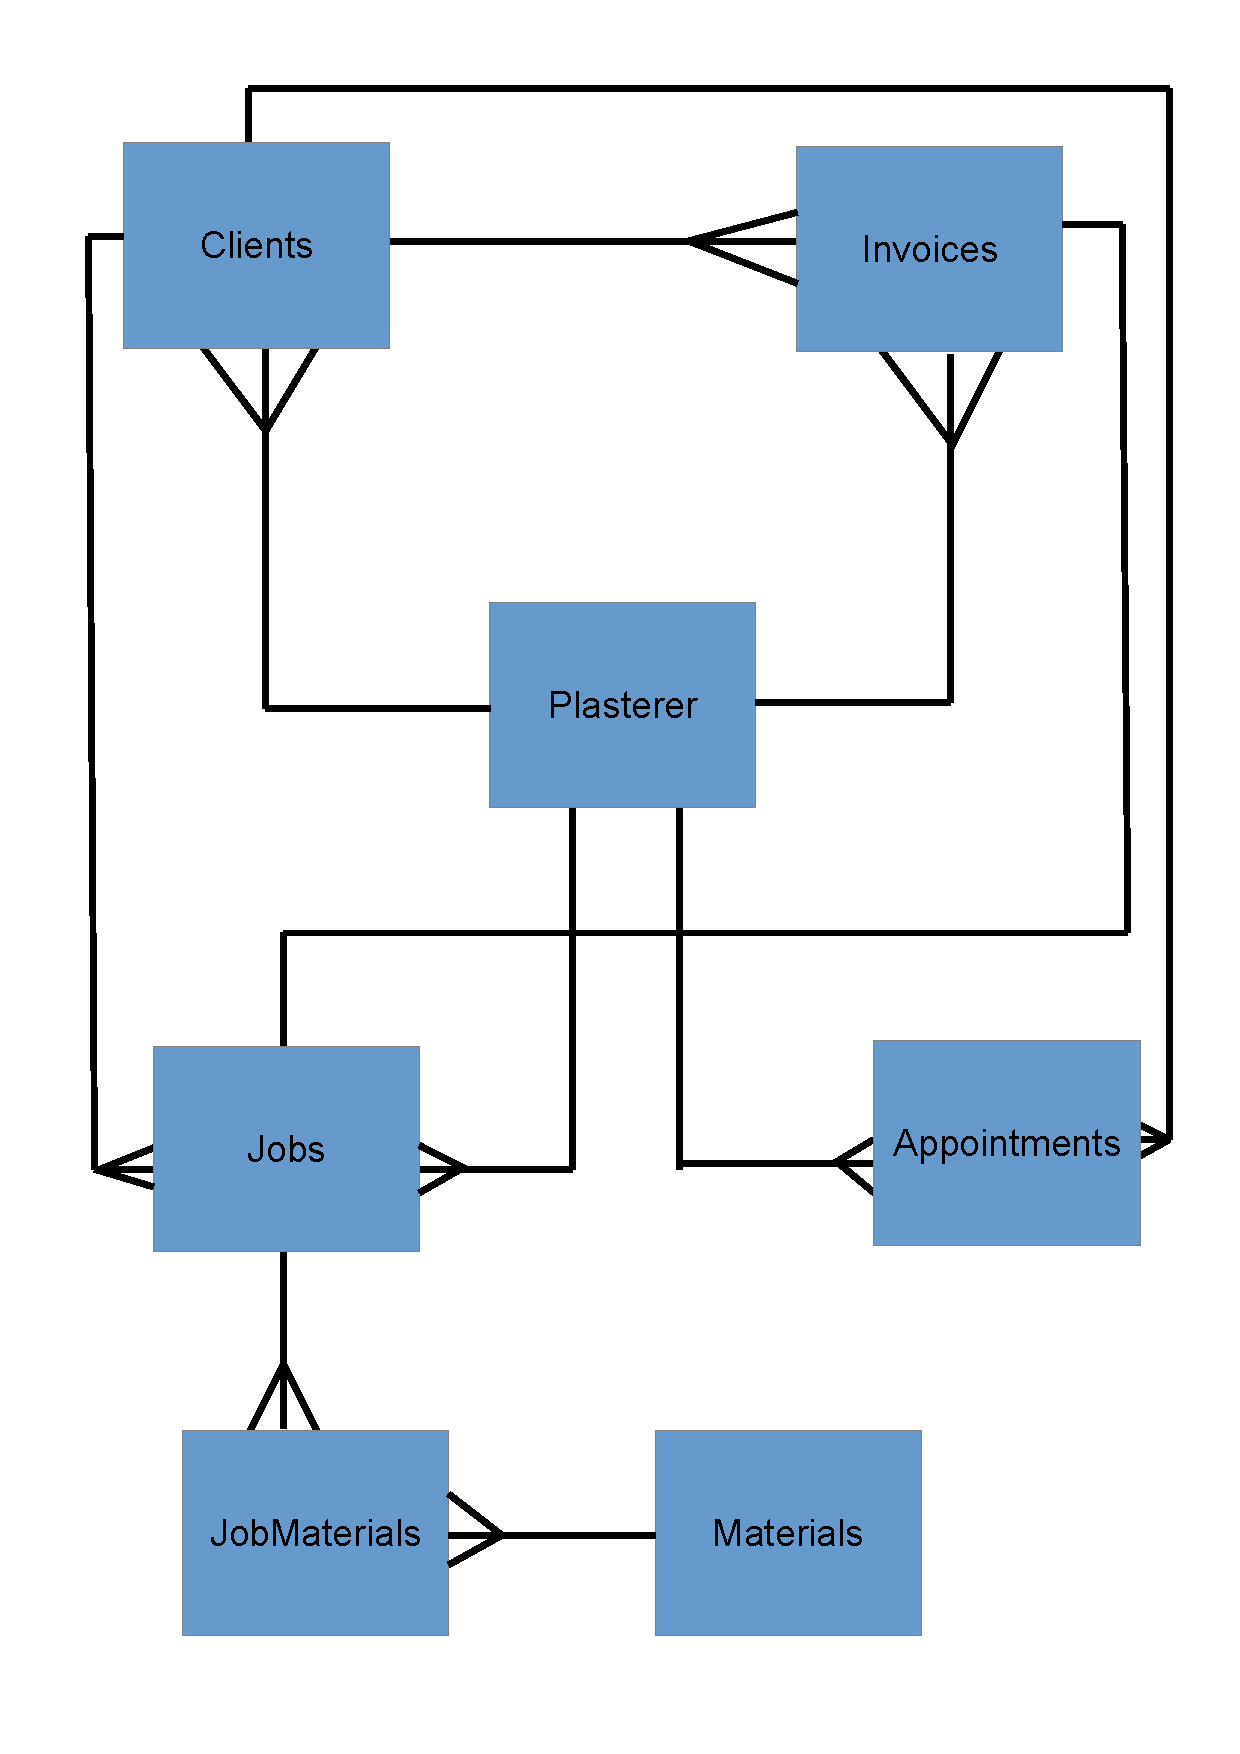
\includegraphics[width=\textwidth]{./Design/images/ERDiagram.pdf}
    \caption{This is the entity relationship diagram for the sqlite3 database.} \label{fig:Entity_Relationship_Diagram}
\end{figure}

\subsubsection{Entity Descriptions}

\begin{flushleft}

Below are the entity descriptions for the various entites in the proposed system. An \underline{underlined} attribute denotes a primary key and a \emph{emphasised}	attribute signifies a foreign key in the entity.

\end{flushleft}




\begin{flushleft}
	\textbf{Client}(\underline{ClientID}, ClientTitle, ClientFirstName, ClientSurname, ClientAddrLine1, ClientAddrLine2, ClientAddrLine3, ClientAddrLine4, ClientEmail, ClientPhoneNumber)
\end{flushleft}



\begin{flushleft}
	\textbf{Plasterer}(\underline{PlastererID}, PlastererFirstName, PlastererSurname, PlastererAddrLine1, PlastererAddrLine2, PlastererAddrLine3, PlastererAddrLine4, PlastererEmail,PlastererPhoneNumber, PlastererDailyRate)
\end{flushleft}



\begin{flushleft}
\textbf{Job}(\underline{JobID}, \emph{ClientID}, \emph{PlastererID}, JobDescription, JobAddrLine1, JobAddrLine2, JobAddrLine3, JobAddrLine4, JobDaysWorked,  JobComplete, \emph{InvoiceID})
\end{flushleft}


\begin{flushleft}
\textbf{Material}(\underline{MaterialID},MaterialName,MaterialPrice)
\end{flushleft}


\begin{flushleft}
\textbf{JobMaterials}(\underline{JobMaterialsID}, \emph{JobID}, \emph{MaterialsID}, JobMaterialsQuantity)
\end{flushleft}


\begin{flushleft}
\textbf{Invoice}(\underline{InvoiceID}, \emph{JobID}, InvoiceAmountPreTax, InvoiceAmountAfterTax, InvoiceReceived, InvoiceDate, InvoiceText, InvoicePaid)
\end{flushleft}



\begin{flushleft}
\textbf{Appointment}(\underline{AppointmentID}, \emph{JobID} AppointmentDate, AppointmentTime)
\end{flushleft}

\subsubsection{1NF to 3NF}
\begin{flushleft}
    \begin{longtable}{|p{12cm}|}
        \hline
			 \textbf{1NF} \\ \hline
         \textbf{Non-Repeating Attributes} \\ \hline
			PersonID (Primary Key) \\ 
         ClientTitle \\
			ClientFirstName \\
			ClientSurname \\
			ClientAddrLine1 \\
			ClientAddrLine2 \\
			ClientAddrLine3 \\
			ClientAddrLine4 \\
			ClientEmail \\
			ClientPhoneNumber \\
			PlastererTitle \\
			PlastererFirstName \\
			PlastererSurname \\
			PlastererAddrLine1 \\
			PlastererAddrLine2 \\
			PlastererAddrLine3 \\
			PlastererAddrLine4 \\
			PlastererEmail \\
			PlastererPhoneNumber \\
			PlastererDailyRate \\ \hline

			\textbf{Repeating Attributes} \\ \hline
			JobID (Primary Key) \\
			PersonID (Composite Key) \\
         JobDescription \\
			JobAddrLine1 \\
			JobAddrLine2 \\
			JobAddrLine3 \\
			JobAddrLine4 \\
			JobDaysWorked \\
			JobComplete \\
			MaterialName \\
			MaterialPrice \\
			JobMaterialsQuantity \\
			InvoiceAmountAfterTax \\
			InvoiceAmountPreTax \\
			InvoiceReceived \\
			InvoiceDate \\
			InvoiceText \\
			InvoicePaid \\
			AppointmentDate \\
			AppointmentTime \\
			AppointmentAddrLine1 \\
			AppointmentAddrLine2 \\
			AppointmentAddrLine3	\\
			AppointmentAddrLine4 \\ \hline
			
    \end{longtable}
\end{flushleft}

\begin{flushleft}
    \begin{longtable}{|p{12cm}|}
        \hline
			 \textbf{2NF} \\ \hline
         \textbf{Group} \\ \hline
			PersonID (Primary Key) \\ 
         ClientTitle \\
			ClientFirstName \\
			ClientSurname \\
			ClientAddrLine1 \\
			ClientAddrLine2 \\
			ClientAddrLine3 \\
			ClientAddrLine4 \\
			ClientEmail \\
			ClientPhoneNumber \\
			PlastererTitle \\
			PlastererFirstName \\
			PlastererSurname \\
			PlastererAddrLine1 \\
			PlastererAddrLine2 \\
			PlastererAddrLine3 \\
			PlastererAddrLine4 \\
			PlastererEmail \\
			PlastererPhoneNumber \\
			PlastererDailyRate \\ \hline

			\textbf{Group} \\ \hline
			JobID (Primary Key) \\
			PersonID (Composite Key) \\
         JobDescription \\
			JobAddrLine1 \\
			JobAddrLine2 \\
			JobAddrLine3 \\
			JobAddrLine4 \\
			JobDaysWorked \\
			JobComplete \\ \hline
		
			\textbf{Group} \\ \hline
			JobID (Primary Key) \\ 
			MaterialName \\
			MaterialPrice \\
			JobMaterialsQuantity \\

			\textbf{Group} \\ \hline
			PersonID (Primary Key) \\
			InvoiceAmountAfterTax \\
			InvoiceAmountPreTax \\
			InvoiceReceived \\
			InvoiceDate \\
			InvoiceText \\
			InvoicePaid \\
			AppointmentDate \\
			AppointmentTime \\
			AppointmentAddrLine1 \\
			AppointmentAddrLine2 \\
			AppointmentAddrLine3	\\
			AppointmentAddrLine4 \\ \hline


    \end{longtable}
\end{flushleft}
\begin{flushleft}
    \begin{longtable}{|p{12cm}|}
                \hline
 			\textbf{3NF} \\ \hline
         \textbf{Group} \\ \hline
			PersonID (Primary Key) \\ 
         ClientTitle \\
			ClientFirstName \\
			ClientSurname \\
			ClientAddrLine1 \\
			ClientAddrLine2 \\
			ClientAddrLine3 \\
			ClientAddrLine4 \\
			ClientEmail \\
			ClientPhoneNumber \\
			PlastererTitle \\
			PlastererFirstName \\
			PlastererSurname \\
			PlastererAddrLine1 \\
			PlastererAddrLine2 \\
			PlastererAddrLine3 \\
			PlastererAddrLine4 \\
			PlastererEmail \\
			PlastererPhoneNumber \\
			PlastererDailyRate \\ \hline

			\textbf{Group} \\ \hline
			JobID (Primary Key) \\
			PersonID (Composite Key) \\
         JobDescription \\
			JobAddrLine1 \\
			JobAddrLine2 \\
			JobAddrLine3 \\
			JobAddrLine4 \\
			JobDaysWorked \\
			JobComplete \\ \hline
		
			\textbf{Group} \\ \hline
			JobID (Primary Key) \\ 
			MaterialID (Foreign Key) \\
			JobMaterialsQuantity \\ \hline


			\textbf{Group} \\ \hline
			MaterialID (Primary Key) \\
			MaterialName \\
			MaterialPrice \\ \hline


			\textbf{Group} \\ \hline
			InvoiceID (Primary Key) \\
			InvoiceAmountAfterTax \\
			InvoiceAmountPreTax \\
			InvoiceReceived \\
			InvoiceDate \\ 
			InvoiceText \\
			InvoicePaid \\	\hline

		\textbf{Group} \\ \hline 
			AppointmentID (Primary Key) \\
			AppointmentDate \\
			AppointmentTime \\
			AppointmentAddrLine1 \\
			AppointmentAddrLine2 \\
			AppointmentAddrLine3	\\
			AppointmentAddrLine4 \\ \hline


			\textbf{Group} \\ \hline
			PersonID (Primary Key) \\
			AppointmentID (Foreign Key) \\
			InvoiceID (Foreign Key) \\ \hline

			
    \end{longtable}
\end{flushleft}




\section{Security and Integrity of the System and Data}

\subsection{Security and Integrity of Data}

\subsection{System Security}

\section{Validation}

\section{Testing}

\begin{landscape}
\subsection{Outline Plan}

\begin{center}
    \begin{tabular}{|p{2cm}|p{5cm}|p{5cm}|p{4cm}|}
        \hline
        \textbf{Test Series} & \textbf{Purpose of Test Series} & \textbf{Testing Strategy} & \textbf{Strategy Rationale}\\ \hline
        Example & Example & Example & Example \\ \hline
    \end{tabular}
\end{center}

\subsection{Detailed Plan}

\begin{center}
    \begin{longtable}{|p{1.5cm}|p{2.5cm}|p{2.5cm}|p{2cm}|p{2cm}|p{2cm}|p{2cm}|p{2cm}|}
        \hline
        \textbf{Test Series} & \textbf{Purpose of Test} & \textbf{Test Description} & \textbf{Test Data} & \textbf{Test Data Type (Normal/ Erroneous/ Boundary)} & \textbf{Expected Result} & \textbf{Actual Result} & \textbf{Evidence}\\ \hline
        Example & Example & Example & Example & Example & Example & Example & Example \\ \hline
    \end{longtable}
\end{center}
\end{landscape}
